%Required for IEEE final version:
%\documentclass[times, 10pt,twocolumn]{article}

%For reviewers
\documentclass[a4paper,11pt]{article}
%\usepackage{doublespace}
\newcommand{\Section}[1]{\section{#1}}
\newcommand{\SubSection}[1]{\subsection{#1}}

\usepackage{times}
%\usepackage{latex8}

%Save some paper, for printing
%\setlength{\topmargin}{-0.7in}
%\setlength{\textheight}{10.2in}
%\setlength{\textwidth}{6.4in}
%\setlength{\oddsidemargin}{-0.1in}
%\setlength{\evensidemargin}{-0.1in}

%My packages
\usepackage{verbatim}
\usepackage{amssymb}
\usepackage{amsmath}
\usepackage{graphicx}
\usepackage{gastex}
\usepackage{multirow}
\usepackage{algorithm}
\usepackage{algorithmic}

%To comment out some parts for submission
\newcommand{\commM}[1]{}
\newcommand{\commE}[1]{#1}

%Frame box for formulas with minipage
\newsavebox{\ffrbox}
\newenvironment{fframe}[2] {\begin{center} \begin{lrbox}{\ffrbox} \begin{minipage}{#1\linewidth} \vspace{#2cm}}{ \end{minipage} \end{lrbox} \fbox{\usebox{\ffrbox}} \end{center}}

%Eigenvalue eigenvector
\newcommand{\vx}[1]{\overrightarrow{x_{#1}}}
\newcommand{\vxe}{\overrightarrow{x^{*}}}
\newcommand{\vxi}[1]{\overrightarrow{x\left(#1\right)}}
\newcommand{\xij}[1]{x\left(#1\right)_{j}}
\newcommand{\vxl}{\vx{\lambda}}
\newcommand{\vxli}[1]{\vx{\lambda_{#1}}}
\newcommand{\vp}{\overrightarrow{p}}

%Matric & vector norms
\newcommand{\nvec}[1]{\lVert #1 \rVert_{v} }
\newcommand{\nmat}[1]{\lVert #1 \rVert_{m} }
\newcommand{\nvece}[1]{\nvec{ #1 }^{2} }
\newcommand{\nvecinf}[1]{\nvec{ #1 }^{\infty} }
\newcommand{\nvecinfal}[1]{\nvec{ #1 }^{{\color[rgb]{0,0,1}\infty}} }
\newcommand{\nmatinf}[1]{\nmat{ #1 }^{\infty} }
\newcommand{\jinlN}[3]{#1 \in #2,..,#3} %\overline{}
\newcommand{\vInd}{\overrightarrow{i_{Ind}}}

%Complexity
\newcommand{\Oc}[1]{\mathcal{O}\left( #1 \right)} %Big o - i.e. time complexity

%Uniformization
\newcommand{\ur}{q} %uniformization rate

%CTMC & DTMC matrices
\newcommand{\mB}{\mP_{B}} %A DTMC where all bad states, i.e. not Phi and not Psi and Psi belonging to some BSCC are made absorbing
\newcommand{\mP}{\mathcal{P}} %A stochastic matrix
\newcommand{\mU}{\mP_{unif}} %Uniformized CTMC
\newcommand{\mT}{\mathcal{T}} %An irreducible submatrix of a stochastic matrix.
\newcommand{\DTMC}{\left( S,\: \mP \right)}
\newcommand{\mQ}{\mathcal{Q}} %Generator matrix
\newcommand{\mR}{\mathcal{R}} %Rate matrix
\newcommand{\CTMC}{\left( S,\: \mQ \right)}
\newcommand{\mA}{\mathcal{A}}
\newcommand{\mQnpvp}{\mQ\left[\npvp \right]}
\newcommand{\mQBnpvp}{\mQ^{B}\left[\npvp \right]}

%CTMC and transient analysis
\newcommand{\pipOti}{\pi^{*} \left(0, t \right )_{i}} %The i'th component of \vpipOt
\newcommand{\vpipOt}{\overrightarrow{\pi^{*} \left(0, t \right )}} % Transient probability, precise
\newcommand{\pipOtj}{\pi^{*} \left(0, t \right )_{j}} % The j'th component of the transient-probability vector, precise
\newcommand{\vpiOt}{\overrightarrow{\pi \left(0, t \right )}} % Transient probability, computed
\newcommand{\piOtj}{\pi \left(0, t \right )_{j}} % The j'th component of the transient-probability vector, computed


\newcommand{\pOi}{p\left( 0 \right)_{i}} % The i'th component of \vpO
\newcommand{\vpO}{\overrightarrow{p \left( 0 \right)} } % Initial distribution for a CTMC
\newcommand{\vpOi}{\overrightarrow{p(0,i)}} %The i'th iteration for uniformized DTMC, with initial distribution \vpiO
\newcommand{\pOij}{p(0,i)_{j}} %The j'th component of \vpOi
\newcommand{\vpOK}{\overrightarrow{p(0,K)}} %The K'th iteration for uniformized DTMC, with initial distribution \vpiO
\newcommand{\pOKj}{p(0,K)_{j}} %The j'th component of \vpOK
\newcommand{\vpOiM}{\overrightarrow{p(0,i+M)}} %The (i+M)'th iteration for uniformized DTMC, with initial distribution \vpiO
\newcommand{\vppO}{\overrightarrow{p^{*}(0)}} %The steady state for transient analysis, starting in state \vpiO
\newcommand{\ppOj}{p^{*}(0)_{j}} %The j'th component of \vppO
\newcommand{\ppOi}{p^{*}(0)_{i}} %The i'th component of \vppO

%CSL model checking
\newcommand{\vis}{\overrightarrow{1_{s} }} %The initial distribution for state s
\newcommand{\vpist}{\overrightarrow{\pi \left( s,t \right) }}
\newcommand{\vpit}{\overrightarrow{\pi \left( t \right) }} %The resulting probability vector for backward computations
\newcommand{\vpsi}{\overrightarrow{p(s,i)}} %An i'th iteration vector for forward computation 
\newcommand{\vpsj}[1]{\overrightarrow{p(s,#1)}} %An j'th iteration vector for forward computation 
\newcommand{\vpsim}{\overrightarrow{p(s,i{+}M)}}  %An (i+m)'th iteration vector for forward computation
\newcommand{\vpOim}{\overrightarrow{p(0,i{+}M)}}  %An (i+m)'th iteration vector for forward computation
\newcommand{\vpsK}{\overrightarrow{p(s,K)}} %A K'th iteration vector for forward computation 
\newcommand{\vpsKI}{\overrightarrow{p(s,K{+}1)}} %A K+1'th iteration vector for forward computation 
\newcommand{\vpi}{\overrightarrow{p(i)}} %An i'th iteration vector for backward computation
\newcommand{\vpK}{\overrightarrow{p(K)}} %An K'th iteration vector for backward computation
\newcommand{\vpKI}{\overrightarrow{p(K{+}1)}} %An K+1'th iteration vector for backward computation
\newcommand{\vpiM}{\overrightarrow{p(i{+}M)}} %An (i+m)'th iteration vector for backward computation
\newcommand{\vpipt}{\overrightarrow{\pi^{*} \left( t \right)}} % A precise solution of equation for backward computations
\newcommand{\vpipst}{\overrightarrow{\pi^{*} \left(s, t \right)}}  % A precise solution of equation for forward computations
\newcommand{\vpps}{\overrightarrow{p^{*}(s)}} % The precise steady-state vector for forward computation
\newcommand{\vpp}{\overrightarrow{p^{*}}} % The precise steady-state vector for backward computation
\newcommand{\vipsi}{\overrightarrow{i_{\Psi}}}
\newcommand{\vibad}{\overrightarrow{i_{\BPsi \cup \SNPhi}}}
\newcommand{\vbpi}{\overrightarrow{p^{B}\left( i \right)}}
\newcommand{\vbpK}{\overrightarrow{p^{B}\left( K \right)}}
\newcommand{\bpij}{p^{B}\left( i \right)_{j}}

\newcommand{\ipsij}{i_{\Psi,j}}  %The j'th component of \vipsi
\newcommand{\pitj}{\pi \left( t \right)_{j}}
\newcommand{\pits}{\pi \left( t \right)_{s}}
\newcommand{\piptj}{\pi^{*} \left( t \right)_{j}}
\newcommand{\pipts}{\pi^{*} \left( t \right)_{s}}
\newcommand{\pistj}{\pi \left(s, t \right)_{j}}
\newcommand{\pipstj}{\pi^{*} \left(s, t \right)_{j}}
\newcommand{\pij}{p(i)_{j}} % The j'th component of the i'th iterate for backward computation
\newcommand{\pilj}{p(i+1)_{j}} % The j'th component of the i+1'th iterate for backward computation
\newcommand{\pKj}{p(K)_{j}} % The j'th component of the K'th iterate for backward computation
\newcommand{\ppj}{p^{*}_{j}} % The j'th component of the precise steady-state vector for backward computation
\newcommand{\psij}{p(s,i)_{j}} % The j'th component of the i'th iterate for forward computation starting from state s
\newcommand{\psji}[2]{p(s,#1)_{#2}} % The i'th component of the j'th iterate for forward computation starting from state s
\newcommand{\pjik}{p(j,i)_{k}} % The k'th component of the i'th iterate for forward computation, starting from state j
\newcommand{\psiNl}{p(s,i)_{N{-}1}} % The N-1'th component of the i'th iterate for forward computation
\newcommand{\psiN}{p(s,i)_{N}} % The N'th component of the i'th iterate for forward computation
\newcommand{\psKNI}{p(s,K)_{N{-}1}} % The N-1'th component of the K'th iterate for forward computation
\newcommand{\psKINI}{p(s,K+1)_{N{-}1}} % The N-1'th component of the K+1'th iterate for forward computation
\newcommand{\psKIN}{p(s,K{+}1)_{N}} % The N'th component of the K+1'th iterate for forward computation
\newcommand{\psKN}{p(s,K)_{N}} % The N'th component of the K'th iterate for forward computation
\newcommand{\psKj}{p(s,K)_{j}} % The j'th component of the K'th iterate for forward computation
\newcommand{\psKZj}{p(s,K{+}Z)_{j}} % The j'th component of the K+Z'th iterate for forward computation

\newcommand{\psKIj}{p(s,K{+}1)_{j}} % The j'th component of the K+1'th iterate for forward computation
\newcommand{\ppsj}{p^{*}(s)_{j}} % The j'th component of the precise steady-state vector for forward computation
\newcommand{\ppsNl}{p^{*}(s)_{N{-}1}} % The N-1'th component of the precise steady-state vector for forward computation
\newcommand{\ppsN}{p^{*}(s)_{N}} % The N'th component of the precise steady-state vector for forward computation

%For the stopping criteria
\newcommand{\psjk}[1]{p\left(s,#1\right)_{k}}
\newcommand{\tmaxk}{t_{k}^{max}}  %the max probability to go from a transient state to and absorbing state k in one step

%Poisson 
\newcommand{\pnd}{e^{-\ur t}\frac{\left( \ur t \right)^{i}}{i!}}
\newcommand{\gpqt}[1]{\gamma_{#1}(t)}
\newcommand{\giqt}{\gpqt{i}}
\newcommand{\gjqt}{\gpqt{j}}

%Fox-Glynn
\newcommand{\ltp}{\mathcal{L}_{\epsilon}} %Left truncation point
\newcommand{\rtp}{\mathcal{R}_{\epsilon}} %Right truncation point
\newcommand{\wi}{w_{i}(t)} %The i'th weight

%Misc
\newcommand{\ToDo}[1]{ 
                                          \begin{center} 
                                          *************************** ToDo ***************************\\
                                          \emph{#1}\\
                                          ************************************************************
                                          \end{center} 
                                        }
\newcommand{\eqnapp}[1]{
                                            \renewcommand{\theequation}{#1.\arabic{equation}}
                                            % redefine the command that creates the equation no.
                                            \setcounter{equation}{0}  % reset counter 
                                          }

%Good and Bad states
	%Sets of states
	\newcommand{\Ind}{Ind} %A set of indexes
	\newcommand{\Gl}{\mathcal{G}} %Goal states
	\newcommand{\Al}{\mathcal{A}} %Allowed states
	\newcommand{\Il}{\mathcal{I}} %Illegal states those which are no \Al and not \Gl
	\newcommand{\Bag}{B_{ \Al, \Gl }} %The bad states to make absorbing
	\newcommand{\vigl}{\overrightarrow{1_{\Gl}}}
	\newcommand{\viind}{\overrightarrow{1_{\Ind}}}
	\newcommand{\AlMBagGl}{\Al \setminus \left( \Gl \cup \Bag \right)}

	%Matrices
	\newcommand{\mQnavg}{\mQ\left[ \Il \cup \Gl \right]}

	%Probabilistic Time reachability
	\newcommand{\PZsf}[3]{\mathrm{P}_{#1}(#2, \:#3)}
	\newcommand{\ppUp}[4]{#1 \: \mathrm{U}^{[#2,#3]} \: #4}
	\newcommand{\PZsaUg}[4]{\PZsf{#1}{#2}{\ppUp{\Al}{#3}{#4}{\Gl}}}
	
	\newcommand{\PZaUg}[3]{\PZf{#1}{\ppUp{\Al}{#2}{#3}{\Gl}}}

	\newcommand{\Psf}[2]{\mbox{\it Prob}(#1, \: #2 )}
	\newcommand{\Pf}[1]{\mathrm{P}( #1 )}
	\newcommand{\PsaUg}[3]{\Psf{#1}{\ppUp{\Al}{#2}{#3}{\Gl}}}
	\newcommand{\PsSUg}[3]{\Psf{#1}{\ppUp{S}{#2}{#3}{\Gl}}}
	
	%Vectors
	\newcommand{\vibadag}{\overrightarrow {i_{\Bag \cup \Il}}}

%PRCTL
\newcommand{\Y}[2]{{\cal Y}^{#1}_{#2}}
\newcommand{\Prob}[3]{{\cal P}_{#1 #2}(#3)}

%CSL
	%Steady-state operator
	 \newcommand{\SpsP}[3]{\mathrm{S}_{\trianglelefteq #1}(#2,\: #3)}
	 
	 %Next operator
	 \newcommand{\Xp}[3]{\mathrm{X}^{[#1,\:#2]} \: #3}
	 
	%Until operator
	\newcommand{\ttUp}[2]{\ppUp{tt}{#1}{#2}{\Psi}}  %The time bounded true Until Psi formula
	\newcommand{\pUp}[2]{\ppUp{\Phi}{#1}{#2}{\Psi}}  %The time bounded Phi Until Psi formula
	
	%Bounded probability and until operator with some initial state
	\newcommand{\PZf}[2]{\mathrm{P}_{#1}(#2)}
	\newcommand{\PZspUp}[4]{\PZsf{#1}{#2}{\pUp{#3}{#4}}}
	\newcommand{\PZsttUp}[4]{\PZsf{#1}{#2}{\ttUp{#3}{#4}}}
	\newcommand{\PZpUp}[3]{\PZf{#1}{\pUp{#2}{#3}}}

	%Probability for state formula with some initial state
	\newcommand{\PspUp}[3]{\Psf{#1}{\pUp{#2}{#3}}}
	\newcommand{\PsttUp}[3]{\Psf{#1}{\ttUp{#2}{#3}}}
	
	%Some bad states, we make absorbing
	\newcommand{\BPsi}{\mathrm{B}_{\Psi}}

%CSRL
	%Until reward operator
	\newcommand{\ppUrp}[6]{#1 \: \mathrm{U}^{{\tiny [#2,#3]}}_{{\tiny [#4,#5]}} \: #6}
	\newcommand{\pUrp}[4]{\ppUrp{\Phi}{#1}{#2}{#3}{#4}{\Psi}}  %The time bounded Phi Until Psi formula

	\newcommand{\npvp}{\lnot \Phi \vee \Psi}
	\newcommand{\Sat}[1]{Sat \left(#1 \right)} % The set of states satisfying \Psi
	\newcommand{\SPsi}{\Sat{\Psi}} % The set of states satisfying \Psi
	\newcommand{\SPhi}{\Sat{\Phi}} % The set of states satisfying \Psi
	\newcommand{\SNPhi}{\Sat{\lnot \Phi}} % The set of states satisfying \not \Psi
	\newcommand{\Bpp}{B_{ \Phi, \Psi }} %The bad states to make absorbing
	\newcommand{\mQB}{\mQ^{B}} %The \mQ[\npvp] matrix with \Bpp states made absorbing

%Tools
	\newcommand{\prism}{\emph{Prism v2.1}}
	\newcommand{\etmcc}{\emph{ETMCC v1.4.2}}
	\newcommand{\mrmc}{\emph{MRMC v1.0}}
	\newcommand{\ultrasan}{\emph{UltraSAN v3.0}}


\newtheorem{theorem}{Theorem}
\newtheorem{prop}[theorem]{Proposition}
\newtheorem{definition}{Definition}
\newtheorem{example}{Example}
\newtheorem{corollary}[theorem]{Corollary}

\newenvironment{proof}{\trivlist \item[\hskip \labelsep{\bf Proof}]}{\hfill\hbox{$\Box$}\endtrivlist}

\pagestyle{empty}

\begin{document}

\title{Safe On-The-Fly Steady-State Detection for \\ Time-Bounded Reachability}

\author{ Joost-Pieter Katoen $^{a,b}$\\
   $^a$
   {\small Software Modeling and Verification Group, RWTH Aachen,}\\
   {\small D-52056 Aachen, Germany,}\\
   {\small Phone: +49 241 8021200, Fax: +49 241 8022217,}\\
   {\small katoen@cs.rwth-aachen.de}\\
 \and
   Ivan S. Zapreev $^b$ \\
   $^b$
   {\small Formal Methods and Tools Group, University of Twente,}\\
   {\small P.O. Box 217, 7500 AE Enschede, The Netherlands,}\\
   {\small Phone: +31 53 4893767, Fax: +31 53 4893247,}\\
   {\small zapreevis@cs.utwente.nl}\\
}

\bibliographystyle{abbrv}

\maketitle
\thispagestyle{empty}

\begin{abstract}
The time-bounded reachability problem for continuous-time Markov chains (CTMCs) amounts 
to determine the probability to reach a (set of) goal state(s) within a given time span, such that 
prior to reaching the goal certain states are avoided. 
Efficient algorithms for time-bounded reachability are at the heart of probabilistic model checkers
such as PRISM and ETMCC.
For large time spans, on-the-fly steady-state detection is commonly applied. 
To obtain correct results (up to a given accuracy), it is essential to avoid detecting premature stationarity. 
This technical report gives a detailed account of criteria for  steady-state detection in the setting of time-bounded reachability. 
This is done for forward and backward reachability algorithms.  
As a spin-off of this study, new results for on-the-fly steady-state detection during CTMC 
transient analysis are reported.  
Based on these results, a precise procedure for steady-state detection for time-bounded 
reachability is obtained.  
Experiments show the impact of these results in probabilistic model checking.
\end{abstract}

\Section{Introduction}
When performing transient analysis for a continuous-time Markov chain (CTMC), it is common practice---in particular in case of large time spans---to use a built-in steady-state detection technique \cite{MalhotraMT_MR94,YounesKNP_STTT05}. 
The underlying idea is to be able to detect whether the CTMC has reached an equilibrium before the finish of the (large) time bound. Whenever such equilibrium is detected, the transient computation can be stopped thus saving expensive computational steps. 
The criteria for detecting such equilibria when guaranteeing an overall inaccuracy of $\varepsilon > 0$ are, however, not always clear and may lead to the detection of premature equilibria. 
This may happen, for instance, when the probability mass in the CTMC under consideration only changes slightly in a series of computational steps due to a ``slow'' movement.

Why is on-the-fly steady-state detection of importance for probabilistic model checking \cite{Kwiatkowska_SLCS03}?
One of the key issues in the model checking of continuous-time probabilistic models such as 
CTMCs is the \emph{time-bounded reachability problem}. 
This entails to determine the probability to reach a (set of) goal state(s) within a given time span, 
such that prior to reaching the goal certain states are avoided. 
This corresponds to a probabilistic variant of time-bounded until formulae as they are used in 
e.g., the verification of timed automata.
For CTMCs, the calculation of such probabilities can be reduced to a transient analysis on a 
modified CTMC \cite{BaierHHK_TSE03}. 
In case of local model checking, a transient analysis needs to be carried out for a single state 
only.
This can be efficiently done in a forward manner, i.e., starting from the state of interest. 
For global model checking, the validity of a logical property needs to be checked in every state 
and thus this probability must be computed for all states. 
Doing so in a backward fashion yields an improvement of ${\cal O}(N)$ over the forward algorithm,
where $N$ is the size of the state space \cite{KatoenKNP_LNCS01}.

As checking time-bounded reachability properties reduces to transient analysis, on-the-fly steady-state detection can be exploited in probabilistic model checking.
Probabilistic model checkers such as PRISM \cite{KwiatkowskaNP_QEST04}, ETMCC \cite{HermansKMS_IJSTTT03} and its variants for stochastic
Petri nets (such as GreatSPN \cite{DAprileDS_DS04} and the APNN Toolbox \cite{BuchholzFKT_MMECCS03}) have adopted this technique
for model checking CSL (Continuous Stochastic Logic \cite{AzizSSB_ACMTCL00,BaierHHK_TSE03}), a variant of CTL.
These model checkers have basically adopted steady-state detection \emph{as it is}, without 
tailoring it to the specific nature of time-bounded reachability.
Other tools that support model checking CSL, such as VESTA \cite{SenVA_CAV05} and Ymer \cite{Younes_CAV05}, use a statistical testing approach and do not support steady-state detection. 

In this report, we present a detailed analysis of the use of on-the-fly steady-state detection in this
setting. 
We start by revisiting and slightly sharpening a (well-known) result by Fox-Glynn \cite{FoxG_ACM88} that is used in computing Poisson probabilities, an essential ingredient in CTMC transient analysis.
Based on this result, we prove criteria to safely decide whether an equilibrium has been reached 
for both the backward and forward reachability algorithm. 
These criteria sharpen known results for on-the-fly steady-state detection for CTMC transient 
analysis \cite{MalhotraMT_MR94} and for CSL model checking \cite{YounesKNP_TACAS04,%
YounesKNP_STTT05}.
Based on these theoretical results, a simple procedure is proposed to safely detect equilibria.
This is done by exploiting the structure of the CTMC that is obtained when reducing time-bounded reachability to transient analysis. 
Experimental results complete this report and show the impact of our theoretical achievements. 
By means of an artificial, though extremely simple CTMC, we show that various existing
probabilistic model checkers detect a premature equilibrium resulting in incorrect verification
results.
We report similar observations for the workstation cluster \cite{HaverkortHK_SRDS00, BuchholzKKT_JLAP03, YounesKNP_TACAS04, KwiatkowskaNP_IMTTCPE02, Prism_WC05}, 
an example that has established itself as a benchmark problem for probabilistic model checking.
(These results confirm a similar phenomenon reported in a recent analysis of the IEEE 802.11 
group communication protocol \cite{MassinkKL_DSN04}.)
Based on these observations, we firmly believe that the results in this technical report improve current
probabilistic model checking technology.

\emph{Organization of the report.} 
Section \ref{s:concepts} introduces relevant concepts of CTMCs and its discrete variant, DTMCs. 
Section \ref{s:fox_glynn_ref} presents the slight refinement of the Fox-Glynn error-bound. 
Section \ref{s:time_b_r} introduces the time-bounded reachability problem, its forward and
backward algorithm, and the use of on-the-fly steady-state detection. 
Sections \ref{s:ss_detect_improved} and \ref{s:osf} contain the main contribution of this report;
these sections present the criteria for detecting equilibria during time-bounded reachability,
and the algorithm to safely detect steady state.    
Section \ref{s:examples} reports on the conducted experiments. Sections \ref{s:timec} and \ref{s:related} talk about algorithms' complexity and related works, and Section \ref{s:concl} concludes.

\Section{Markov chain preliminaries \label{s:concepts}}

		This section recalls stationary probabilities for DTMCs, transient probabilities of CTMCs, and some related concepts.   For more information we refer to standard textbooks on Markov chains \cite{Tijms_03, Haverkort_98}.  Let $S = \left\{1, \ldots,N \right\}$ be a finite set of state indexes with $|S|=N$.
	
\SubSection{Discrete-time Markov chains}

		\begin{definition}
			A Discrete-time Markov Chain (\emph{DTMC}) is a tuple $\DTMC$ with finite set $S$ of states and state-transition probability matrix $\mP : S \times S \rightarrow \left[0,\:1 \right]$, where $\mP=\left(p_{i,j}\right)$ and $\forall i \in S : \sum_{j \in S} p_{i,j}=1$.
		\end{definition}
		
		The matrix entry $p_{i,j}$ denotes the probability to move from state $i$ to state $j$ in one step.  Let $\vpO$ denote the initial probability distribution of $\DTMC$, i.e., $\pOi$ denotes the probability to be initially in state $i$.

		\begin{definition}
		The \emph{limiting} state-probability of  DTMC $\DTMC$ is a vector $\vppO$ such that:
			\begin{equation}
				\vppO = lim_{n \to \infty} \: \vpO \cdot \mP^{n}
				\label{eq:ssl_dtmc}
			\end{equation}
		\end{definition}
		
		Whenever this limit exists, it can be obtained by solving the system of linear equations:
		
		\begin{equation}
			\vp = \vp \cdot \mP \text{, }\sum_{i \in S} p_{i} = 1
			\label{eq:sse_dtmc}
		\end{equation}
				
		In case the limit (\ref{eq:ssl_dtmc}) does not exist, the equation (\ref{eq:sse_dtmc}) may still have a solution.  The solution of equation (\ref{eq:sse_dtmc}) is also known as \emph{stationary} or \emph{steady-state} distribution.	
		In general, the limiting state-probability $\ppOj$ can be interpreted either as the proportion of time the DTMC is in state $i$ on the long run or, alternatively, as the probability that the DTMC is in state $i$ when taking a snapshot after a long time.  The vector $\vp$ in equation (\ref{eq:sse_dtmc}) is the left eigenvector of $\mP$ that corresponds to the unit eigenvalue.  As $\mP$ is a stochastic matrix, $\mP$ always has a unit eigenvalue, and no other eigenvalue exceeds it in modulus.  The following theorem, see \cite{Haverkort_98} for details, states when a DTMC has a unique limiting state-distribution.
		
		\begin{theorem}
			An irreducible and aperiodic finite DTMC has a unique limiting distribution (\ref{eq:ssl_dtmc}).  This distribution coincides with the steady-state distribution and does not depend on the initial distribution $\vpO$.
		\end{theorem}
		
		Informally, \emph{irreducible} means that every state is reachable from every other state, (i.e. the underlying graph is strongly connected).  A DTMC is periodic if one of its states is periodic.  State $i$ is periodic if for some $d > 1$ it holds that the probability to return to state $i$ in $n$ steps is 0, for all $n$ such that $n \mbox{ \sl mod } d \neq 0$.  A sufficient condition for an irreducible DTMC to be \emph{aperiodic} is that there exists at least one state with a self loop. A possible way to determine the steady-state probabilities for a DTMC is to compute the dominant (eigenvalue, eigenvector) pair of $\mP$.  This is described in the following.
		
		\paragraph{The Power method. \label{sss:power_method}}
		The Power method \cite{Stewart_94} is a well-known numerical technique for computing the dominant eigenvalue and its corresponding eigenvector for an arbitrary matrix $\mA$  of cardinality $N \times N$.  It is described by the following iterative procedure, for $m \geq 1$:
		
		\begin{equation}
			\vxi{m}	= \frac{1}{ \nvecinf{ \vxi{m{-}1}{\cdot}\mA } }\vxi{m{-}1} \cdot \mA
		\end{equation}
		
		Where $\vxi{0}$ is an arbitrary initial vector, and $\nvecinf{.}$ is the l-infinity vector norm. This iteration converges to the eigenvector $\vxli{1}$ corresponding to the dominant eigenvalue $\lambda_{1}$, provided the following conditions hold:

		\begin{enumerate}
			\item Matrix $\mA$ has $N$ independent left (right) eigenvectors $\left\lbrace \vxli{i} \right\rbrace $
			\item The eigenvalues can be ordered by magnitude: 
					\begin{center}
						$\left\| \lambda_{1} \right\| > \left\| \lambda_{2} \right\| \geq \left\| \lambda_{3} \right\| \ldots \geq \left\| \lambda_{N} \right\|$
					\end{center}
		\end{enumerate}
		The convergence rate of the Power method is $\frac{\lambda_{2}}{\lambda_{1}}$ where  $\lambda_{1}$ and $\lambda_{2}$ are dominant and subdominant eigenvalues.
In case of a stochastic matrix $\mP$, the dominant eigenvalue is $1$ and the iterative procedure reduces to:

		\begin{equation}
			\vxi{m}	= \vxi{m{-}1}{\cdot}\mP
		\end{equation}

		If the matrix $\mP$ is aperiodic, convergence of the Power method is guaranteed.  If, in addition, $\mP$ is irreducible, then the result of the power iterations will not depend on the initial vector $\vxi{0}$.

		According to \cite{Stewart_94}, the number $K$ of iterations required to satisfy a tolerance criterion $\varepsilon > 0$ for the Power method may be approximately obtained as:
	
		\begin{equation}
			K = \dfrac{\log_{2} \varepsilon}{\log_{2} | \lambda_{2} |}
		\end{equation}
	
		In practice however, $ \lambda_{2}$ is difficult to compute, and other convergence tests are used \cite{Stewart_94}, such as for $M > 0$:
		\begin{enumerate}
			\item An absolute convergence test: \[\nvec{\vxi{i} - \vxi{i{+}M}} < \varepsilon\]
			\item A relative convergence test: \[\max_{\jinlN{j}{1}{N}} \left( \frac{ | \xij{i{+}M} - \xij{i} |}{ | \xij{i{+}M} |} \right) < \varepsilon\]
		\end{enumerate}

		In general, $M$ is a function of the convergence rate and the iteration index $i$, but may be taken as constant.
		Unfortunately, none of these tests gives a precise estimate.  Stewart \cite{Stewart_94} therefore suggests to envisage a \emph{battery} of convergence tests, all of which must be satisfied before the approximation is accepted as being sufficiently accurate.

	\SubSection{Transient and stationary probabilities of CTMCs}
		
		\begin{definition}
			A Continuous-time Markov Chain (\emph{CTMC}) is a tuple $\CTMC$ with finite set $S$ of states and generator matrix $\mQ : S \times S \rightarrow \mathcal{R}$, where $\mQ=\left(q_{i,j}\right)$, $\forall i,j \in S : i \neq j : q_{i,j} \geq 0$, and $\forall i \in S : q_{i,i} = - \sum_{j \in S, \: i \neq j} q_{i,j}$. 
		\end{definition}
		
		Let us explain the intuitive meaning of $q_{i,j}$.  In a CTMC, state residence times are exponentially distributed.  More precisely, the time spent in state $i$ is governed by a negative exponential distribution with rate $|q_{i,i}|$.  The rate $|q_{i,i}|$ thus specifies the total rate to leave state $i$.  On leaving state $i$, a discrete probabilistic choice takes place among all possible successors, i.e. all states $j$ for which $q_{i,j} > 0$.  The probability to move to state $j$ is defined as $q_{i,j} / |q_{i,i}|$.  The transient probabilities of CTMC $\CTMC$ are defined by the following differential equation:
		  \begin{equation}
			\frac{d \vpipOt}{dt} = \vpipOt \cdot \mQ \nonumber
		  \end{equation}
		The solution of this differential equation system is given by:
		
		\begin{equation}
			\vpipOt = \vpO \cdot e^{\mQ{\cdot}t}
			\label{eq:transient}
		\end{equation}
		Here, $\vpipOt$ defines the state-probability after a delay of $t$ time-units given that  $\vpO$ is the initial distribution.  $\pipOti$ thus is the probability to be in state $i$ after $t$ time-units given $\vpO$.

	\paragraph{The stationary probability of a CTMC}
		The stationary (steady-state) probabilities for a CTMC are a solution of the following system of linear equations:
		\begin{equation}
			\overrightarrow{p} {\cdot} \mQ = \overrightarrow{0}, \quad \text{where} \quad \sum_{i \in S} p_{i} = 1
			\label{eq:sse_cmtc}
		\end{equation}
		A solution of equation (\ref{eq:sse_cmtc}) may be found by alternatively presenting it as the following unit eigenvalue problem \cite{Stewart_ACM78}:
		\begin{equation}
			\overrightarrow{p}{\cdot}\mP = \overrightarrow{p}
			\label{eq:sse_u_ctmc}
		\end{equation}
		where $\mP=\frac{\mQ}{\ur}+\mathcal{I}$ and $\ur \geq \max_{i \in S}| q_{i,i} |$.  It is well known \cite{Stewart_ACM78} that if
		\begin{equation}
			\ur > \max_{i \in S} |q_{i,i}|
			\label{eq:unif_rate}
		\end{equation}
		then all eigenvalues, except the unit eigenvalue, are strictly less than unity in modulus, which makes DTMC $\mP$ aperiodic.

	\paragraph{Jensen's method}
		 Jensen's method, also known as uniformization, replaces $\mQ$ by $\mP$ in equation (\ref{eq:transient}).  Expanding the matrix exponent according to Taylor-McLaurin yields:

		\begin{equation}
			\vpipOt = \sum_{i=0}^{\infty}\giqt {\cdot} \vpOi
			\label{eq:transient_2}
		\end{equation}

		where $\giqt = \pnd$ is the Poisson density function, $\vpOi = \vpO {\cdot} \mP^{i}$, and $\ur$ is the \emph{uniformization rate}.

	\SubSection{On-the-fly steady-state detection \label{ss:ofssd_trans}}
		Equation (\ref{eq:transient_2}) contains $\vpO \cdot \mP^{i}$ which is the power iteration for the DTMC $\mP$, and that is where the steady-state detection comes into play.  Malhotra \emph{et al.} \cite{MalhotraMT_MR94} present a numerical method, which takes into account steady-state detection, for computing CTMC transient probabilities (see equation (\ref{eq:transient_2})) with an overall error bound $\varepsilon$.  For the sake of this technical report, we state their result in the following form:

		\begin{theorem}
			Let $\DTMC$ be an aperiodic DTMC with initial distribution $\vpO$ and steady-state distribution $\vppO$. If for some $K$ and $\delta > 0$ it holds that $\forall i \geq K : \nvec{\vppO - \vpOi} \leq \delta$, where $\nvec{.}$ is an arbitrary vector norm \footnote{It should be noted that Theorem \ref{th:error_fwd_initial} does not hold for an arbitrary norm $\nvec{.}$. In fact, an additional  condition is required, that is $\nvec{\vp}\leq 1$ for any distribution vector $\vp$.}, then for
			\begin{equation}
				\vpipOt = \sum_{i=0}^{\infty}\giqt \vpOi \nonumber
			\end{equation}
			and for inaccuracy $\varepsilon > 0$:
			\begin{equation}
				\displaystyle
				\vpiOt = \left\{
				\begin{array}{ll}
					\vpOK & \text{, if } K < \ltp\\
					\sum_{i=\ltp}^{K}\giqt \vpOi + \vpOK \left(1- \sum_{i=0}^{K}\giqt \right) & \text{, if } \ltp \leq K \leq \rtp\\
					\sum_{i=\ltp}^{\rtp}\giqt \vpOi & \text{, if } K > \rtp\\
				\end{array}
				\right .
				\label{eq:ssd_LR_initial}
			\end{equation}
			the following inequality holds:
			\begin{equation}
				\nvec{\vpipOt - \vpiOt} \ \leq \ 2 \delta + \frac{\varepsilon}{2} \nonumber
			\end{equation}
			Here, $\ltp$ and $\rtp$ are computed using the Fox-Glynn algorithm (see below), such that $\sum_{i=0}^{\ltp-1} \giqt \leq \frac{\varepsilon}{2}$, and $\sum_{i=\rtp+1}^{\infty} \giqt \leq \frac{\varepsilon}{2}$.
			\label{th:error_fwd_initial}
		\end{theorem}
		
		Theorem \ref{th:error_fwd_initial} can now be used to obtain a criterion for guaranteeing an overall inaccuracy of $\varepsilon > 0$ for transient analysis with on-the-fly steady-state detection.  This is stated by the following corollary.
		
		\begin{corollary}
			Under the same conditions as Theorem \ref{th:error_fwd_initial}: 
				\begin{equation}
					\nvec{\vppO - \vpOK} \leq \frac{\varepsilon}{4} \text{ implies } \nvec{\vpipOt - \vpiOt} \leq \varepsilon
					\label{eq:malh_cr_cor}
				\end{equation}
			\label{cl:error_fwd_initial}
 		\end{corollary}

		As $\nvec{\vppO - \vpOK}$ is not known during computations (since $\vppO$ is unknown, and typically not computed a priori as this is computationally too expensive), \cite{MalhotraMT_MR94} suggests to use the absolute convergence test.  This amounts to replace the premise in equation (\ref{eq:malh_cr_cor}) by:
		\begin{equation}
			\nvec{\vpOi - \vpOiM} \leq \frac{\varepsilon}{4} \quad \mbox{for } M > 0 \label{eq:malh_cr}
		\end{equation}
		Accordingly, $\vpOK$ with $K = i{+}M$ is used as an approximation of the real steady-state distribution.  This approach thus boils down to comparing probability vectors that are $M$ iterations apart.  Once these $M$-apart probability vectors are close enough, it is assumed that the CTMC has reached an equilibrium.  This approach, of course, has the drawback that due to the use of an approximation of the stationary probability, an equilibrium may be detected prematurely.  A detailed analysis revealed that in deriving the above result in \cite{MalhotraMT_MR94},  an important ingredient of the Fox-Glynn algorithm is not considered, viz.\ the so-called weights.  (Weights will be discussed in detail in the next section).   It will be shown in the remainder of this report that weights play an important role to obtain \emph{safe} criteria for detecting equilibria.

\Section{Fox-Glynn error bound revisited \label{s:fox_glynn_ref}}
	
	Recall that  $\giqt = \pnd$ is a Poisson density function, thus $\sum_{i=0}^{\infty}\giqt = 1$.  $\giqt$ denotes the probability that $i$ events occur in a period of $t$ time units, given that the average rate of events is $q$.  The particular shape of the Poisson density function (for an example see Figure \ref{fig:poisson}) allows for ignoring the ``tails'' of the density function.  For a given error bound $\varepsilon > 0$, these so-called left and right \emph{truncation points} are given by $\ltp$ and $\rtp$ such that:
	$$ \sum_{i=0}^{\ltp{-}1}\giqt \leq \frac{\varepsilon}{4} \text{, and} \sum_{i=\rtp{+}1}^{\infty}\giqt \leq \frac{\varepsilon}{4} \quad .$$
	For real-valued function $f : \mathbb{N} \to \mathbb{R}$, the Fox-Glynn algorithm \cite{FoxG_ACM88} allows to compute
	\begin{equation}
	 	\sum_{i=0}^{\infty} \giqt f(i) \approx \frac{1}{W}\sum_{i = \ltp}^{\rtp} \wi f(i) \nonumber
	 \end{equation}
	 where $\wi = \alpha \giqt$ for some constant $\alpha \neq 0$ are \emph{weights}, and $W = \sum_{i=\ltp}^{\rtp} \wi$ is a normalization weight.  Note the resemblance of the left-hand side of the last equation and equation (\ref{eq:transient_2}).  The weights $\wi$ and the normalization weight $W$ are used to prevent underflows and are computed; $\alpha$ is an unknown constant.
	
	\begin{figure}[ht!]
		\begin{center}
			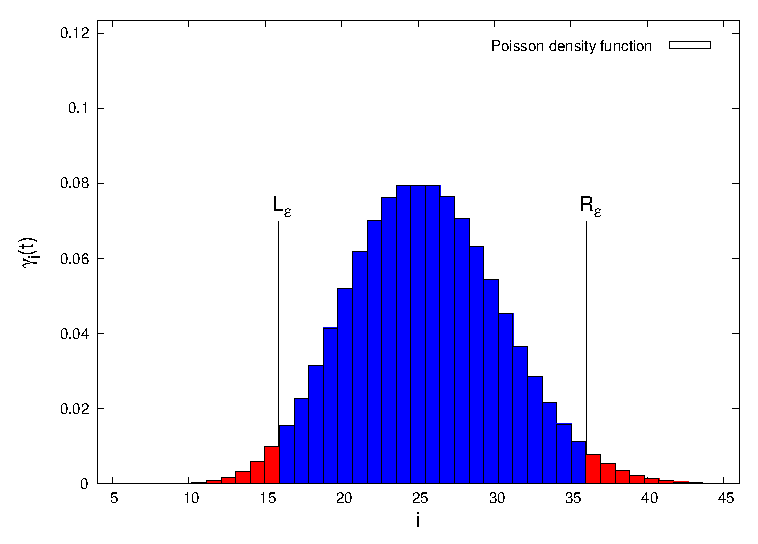
\includegraphics[scale=0.5, angle=0]{./poisson.eps}
		\end{center}
		\caption{Poisson density function with $qt=2$ and $\rtp$ \label{fig:poisson}}
	\end{figure}
	
	\begin{prop}
		\cite{FoxG_ACM88} For real-valued function $f$ with $\|f\| = \sup_{i \in \mathbb{N}}|f(i)|$ and $\sum_{i=\ltp}^{\rtp} \giqt \geq 1 - \frac{\varepsilon}{2}$ it holds:
		\begin{equation}
			\left| \sum_{i=0}^{\infty} \giqt f(i) - \frac{1}{W}\sum_{i = \ltp}^{\rtp} \wi f(i) \right| \leq \varepsilon \cdot \|f\| \quad . \nonumber
		\end{equation}
	\end{prop}
	The following refinement can be made for the case when $f$ does not change sign, i.e., $f(i) \leq 0$ or $f(i) \geq 0$, for all $i$.
	\begin{prop}
		For real-valued function $f$ that does not change sign with $\|f\| = \sup_{i \in \mathbb{N}}|f(i)|$ and $\sum_{i=\ltp}^{\rtp} \giqt \geq 1 - \frac{\varepsilon}{2}$ it holds:
		\begin{equation}
			\left| \sum_{i=0}^{\infty} \giqt f(i) - \frac{1}{W}\sum_{i = \ltp}^{\rtp} \wi f(i) \right| \leq \frac{\varepsilon}{2} \cdot \|f\| \quad . \label{eq:fg_imp}
		\end{equation}
			\label{pr:fg_imp}
	\end{prop}
	\begin{proof}
		Initially we have:
		
		\begin{minipage}[t]{0.45\linewidth}
			\begin{eqnarray}
				\sum_{i=\ltp}^{\rtp} \giqt \geq 1 - \frac{\varepsilon}{2} \label{eq:init_1} \\
				\forall i \in \mathbb{N} : \giqt > 0 \label{eq:init_3}
			\end{eqnarray}
		\end{minipage} \hfill
		\begin{minipage}[t]{0.45\linewidth}
			\begin{eqnarray}
				\sum_{i=0}^{\infty} \giqt = 1 \label{eq:init_2} \\
				\|f\| = \sup_{i \in \mathbb{N}}|f(i)| \label{eq:init_4}
			\end{eqnarray}
		\end{minipage}
		
		Distinguish two cases:
		\begin{equation}
			\forall i \in \mathbb{N} : 0 \leq f(i) \leq \|f\| \text{, $f$ is non-negative} \label{eq:funct_pos}
		\end{equation}
		\begin{equation}
			\forall i \in \mathbb{N} : -\|f\| \leq f(i) \leq 0 \text{, $f$ is non-positive} \label{eq:funct_neg}
		\end{equation}
				  
		Let $\beta = \sum_{i=\ltp}^{\rtp} \giqt$.  We obtain from (\ref{eq:init_2}):
		\begin{equation}
			1 - \beta = \sum_{i = 0}^{\ltp-1} \giqt + \sum_{i = \rtp+1}^{\infty} \giqt \label{eq:beta_3}
		\end{equation}
		
		Using (\ref{eq:init_1}), (\ref{eq:init_2}), and (\ref{eq:init_3}) it follows $1- \frac{\varepsilon}{2} \leq \beta \leq 1$, or equivalently:

		\begin{minipage}[t]{0.45\linewidth}
			\begin{equation}
				- \frac{\varepsilon}{2} \leq \beta -1 \leq 0  \label{eq:beta_1}
			\end{equation}
		\end{minipage} \hfill
		\begin{minipage}[t]{0.45\linewidth}
			\begin{equation}
				0 \leq 1- \beta \leq \frac{\varepsilon}{2} \label{eq:beta_2}
			\end{equation}
		\end{minipage}

		Notice that
		\begin{eqnarray}
			\sum_{i=0}^{\infty} \giqt f(i) - \frac{1}{W}\sum_{i = \ltp}^{\rtp} \wi f(i) = \nonumber \\
			\underbrace{\sum_{i = 0}^{\ltp-1} \giqt f(i) + \sum_{i = \rtp+1}^{\infty} \giqt f(i)}_{ = A} +  
			\underbrace{\sum_{i = \ltp}^{\rtp} \left( \giqt - \frac{\wi}{W} \right) f(i)}_{ = B} \nonumber
		\end{eqnarray}
		
		If $f$ is non-negative, from (\ref{eq:funct_pos}), (\ref{eq:beta_3}), and (\ref{eq:beta_2}) one can easily obtain:
		\begin{equation}
			0 \leq A \leq \frac{\varepsilon}{2} \cdot \|f\|
			\label{eq:fg_A_pos}
		\end{equation}
		
		Similarly, from (\ref{eq:beta_1}), (\ref{eq:funct_pos}) and the definition of $\beta$ it follows that:
		\begin{equation}
			- \frac{\varepsilon}{2} \cdot \|f\| \leq B \leq 0
			\label{eq:fg_B_pos}
		\end{equation}
		
		This follows from the following facts:
		\begin{eqnarray}
			B = \sum_{i = \ltp}^{\rtp} \left( \giqt - \frac{\alpha \giqt }{\sum^{\rtp}_{i=\ltp} \alpha \giqt} \right) f(i) = \nonumber \\
			\sum_{i = \ltp}^{\rtp} \giqt \left( 1 - \frac{1}{\sum^{\rtp}_{i=\ltp} \giqt} \right) f(i) = \frac{\beta - 1}{\beta} \sum_{i = \ltp}^{\rtp} \giqt  f(i)\nonumber
		\end{eqnarray}
		
		and
		\begin{equation}
			- \frac{\varepsilon}{2} \cdot \|f\| = - \frac{\varepsilon}{2} \cdot \|f\|\cdot \frac{1}{\beta} \sum_{i = \ltp}^{\rtp} \giqt \leq \frac{\beta - 1}{\beta} \sum_{i = \ltp}^{\rtp} \giqt  f(i) \leq 0
		\end{equation}  

		Symmetrically, if $f$ is non-positive, from equations (\ref{eq:funct_neg}), (\ref{eq:beta_3}), and (\ref{eq:beta_2}) one can easily obtain:
		\begin{equation}
			- \frac{\varepsilon}{2} \cdot \|f\| \leq A \leq 0
			\label{eq:fg_A_neg}
		\end{equation}
		
		Similarly, from (\ref{eq:beta_1}), (\ref{eq:funct_neg}) and the definition of $\beta$ it follows that
		\begin{equation}
			0 \leq B \leq \frac{\varepsilon}{2} \cdot \|f\|
			\label{eq:fg_B_neg}
		\end{equation}
		
		Finally, summing up inequalities (\ref{eq:fg_A_pos}) and (\ref{eq:fg_B_pos}) for non-negative $f$, or (\ref{eq:fg_A_neg}) and (\ref{eq:fg_B_neg}) for non-positive $f$, we obtain:
		\begin{equation}
			- \frac{\varepsilon}{2} \cdot \|f\| \leq \sum_{i=0}^{\infty} \giqt f(i) - \frac{1}{W}\sum_{i = \ltp}^{\rtp} \wi f(i) \leq \frac{\varepsilon}{2} \cdot \|f\| \nonumber
		\end{equation}
		
		for any $f$ that does not change sign.  This proves the claim.
	\end{proof}

\Section{Time-bounded reachability \label{s:time_b_r}}

		A recent popular approach to analyze properties of Markov chains is probabilistic model checking; for an overview see \cite{Kwiatkowska_SLCS03}.  Time-bounded reachability is at the heart of model-checking algorithms for CTMCs.  Let us explain this problem by means of an example. Consider a CTMC with many states among which some illegal (or: forbidden) states and some goal states.  Suppose we are interested in determining the states from which a goal state may be reached with a high probability, say at least $0.92$, within time interval $[0,14.5]$, while never visiting an illegal state before reaching its goal. We thus consider scenarios in which the system starts in some state $s \in S$, visits any number of states which are not illegal, while finally ending up in some goal state.  In the logic CSL~\cite{AzizSSB_ACMTCL00,BaierHHK_TSE03}, a continuous-time probabilistic extension of CTL,  this requirement is formulated by:
		\begin{equation}
			\PZaUg{\geq 0.92}{0}{14.5} \nonumber
		\end{equation}
		where $\Al$ denotes the set of legal (allowed) states and $\Gl$ denotes the set of goal states.\footnote{In logical formulas, we identify set $\Al$. with its characteristic function.}
		
		The part between parentheses characterizes a set of paths, where a single path is an alternating sequence $s_{0}t_{0}s_{1}t_{1}s_{2}t_{2}\ldots$ where $t_{j} > 0$ denotes the residence time in state $s_{j}$, and $s_{0} = s$.  Such path satisfies $\ppUp{\Al}{0}{14.5}{\Gl}$ if there exists an index $j \geq 0$ such that $s_{j} \in \Gl$, $s_i \in \Al$ for all $i < j$, and $s_{j}$ is reached within $14.5$ time units, i.e., $\sum_{i=0}^{j{-}1}t_{i} \leq 14.5$.  For the sake of brevity, we do not present the detailed semantics of this operator; these details can be found in \cite{AzizSSB_ACMTCL00,BaierHHK_TSE03}.
	
		Time-bounded reachability thus amounts to compute $\PsaUg{s}{0}{t}$, the probability for state $s$ satisfying formula $\ppUp{\Al}{0}{t}{\Gl}$.  This problem can be reduced to the computation of transient probabilities in a modified CTMC \cite{BaierHHK_TSE03}.  This goes as follows.  In the original CTMC $\CTMC$, all states in $\Gl$ and all states that are neither in $\Al$ nor in $\Gl$ are made absorbing, i.e., their outgoing transitions are removed.   This operation is formally defined by:
		\begin{definition}
		For CTMC $\CTMC$ and $S' \subseteq S$ let CTMC $(S, \mQ')$  be obtained by making all states in $S'$ absorbing, i.e., $\mQ' = \mQ[S']$ where $q'_{i,j} = q_{i,j}$ if $i \not\in S'$ and 0 otherwise.
		\end{definition}
	
		Note, that in order to make a state $s$ in a DTMC absorbing, all outgoing transitions of $s$ are removed and $s$ is equipped with a self-loop (with probability 1).  In a CTMC, it suffices to remove the outgoing transitions.  It now follows that:
		$$
			\PsaUg{s}{0}{t} \mbox{ in } \CTMC \ = \  \PsSUg{s}{t}{t} \mbox{ in } (S, \mQnavg) \mbox{ where }   \Il=S \setminus \left( \Al \cup \Gl\right)
		$$
		
		For any state $s \in S$, the probability $\PsaUg{s}{0}{t}$ can be computed using Algorithm \ref{alg:fwd}, where the matrix exponent can be computed numerically using uniformization and $\vis$ is the initial distribution for the case when starting in state $s$.
		\begin{algorithm}
			\caption{Computing $\PsaUg{s}{0}{t}$ in a ``forward'' manner}
			\label{alg:fwd}
			\begin{algorithmic}[1]
				\STATE Determine $\mQnavg$
				\STATE Compute $\vpipst = \vis \cdot e^{\mQnavg t}$
				\STATE Return $\PsaUg{s}{0}{t} = \sum_{j \in \Gl}\pipstj$
			\end{algorithmic}
		\end{algorithm}
		\cite{KatoenKNP_LNCS01} suggests an improvement of this method (cf.\ Algorithm \ref{alg:bwd}).  Like before, the matrix exponent is computed using uniformization.  Let $\vigl$ be the characteristic vector of the set $\Gl$.

		\begin{algorithm}
			\caption{Computing $\PsaUg{s}{0}{t}$ in a ``backward'' manner}
			\label{alg:bwd}
			\begin{algorithmic}[1]
				\STATE Determine $\mQnavg$
				\STATE Compute $\vpipt = e^{\mQnavg t} \cdot \vigl$
				\STATE Return $\forall \jinlN{s}{1}{N} : \PsaUg{s}{0}{t} = \pipts$
			\end{algorithmic}
		\end{algorithm}
	
	\SubSection{On-the-fly steady state detection  \label{ss:ussd}}
		The steady-state detection for transient analysis of CTMCs discussed in Section \ref{ss:ofssd_trans}, is applicable to the forward computations in a straightforward way. Steady-state detection for backward computations has been recently discussed in \cite{YounesKNP_STTT05}.  The approach by Younes \emph{et al.} is based on the following result.

		\begin{theorem}
			Let $\DTMC$ be an aperiodic DTMC with $\Ind \subseteq S$ such that $\forall j \in \Ind : P(j,j) = 1$, $\vpi=\mP^{i} \cdot \viind$ and steady-state vector $\vpp$. If for some $K$ and $\delta > 0$ it holds that $\forall i \geq K:\nvec{\vpp - \vpi} \leq \delta$, then for
			\begin{equation}
				\vpipt = \sum_{i=0}^{\infty}\giqt \vpi \nonumber
			\end{equation}
			and for inaccuracy $\varepsilon > 0$:
			\begin{equation}
				\displaystyle
				\vpit = \left\{
				\begin{array}{ll}
					\vpK & \text{, if } K < \ltp\\
					\sum_{i=\ltp}^{K}\giqt \vpi + \vpK \left(1- \sum_{i=\ltp}^{K}\giqt \right) & \text{, if } \ltp \leq K \leq \rtp\\
					\sum_{i=\ltp}^{\rtp}\giqt \vpi & \text{, if } K > \rtp\\
				\end{array}
				\right .
				\label{eq:ssd_LR_b}
			\end{equation}
			the following inequality holds:
			\begin{equation}
				\nvec{ \vpipt - \vpit } \leq 2 \delta + \frac{\varepsilon}{2} \nonumber
			\end{equation}
			Here $\ltp$, and $\rtp$ are computed using the Fox-Glynn algorithm, such that $\sum_{i=0}^{\ltp{-}1} \giqt \leq \frac{\varepsilon}{2}$ and $\sum_{i=\rtp{+}1}^{\infty} \giqt \leq \frac{\varepsilon}{2}$.
			\label{th:error_bwd_initial}
		\end{theorem}
		In \cite{YounesKNP_STTT05}, this result has led to the following practical check for steady-state:
		%\begin{corollary}
			%Under the same conditions as Theorem \ref{th:error_bwd_initial}:
			\begin{equation}
				\nvec{\vpp - \vpK} \leq \frac{\varepsilon}{8} \text{ implies } \forall j \in S : -\frac{\varepsilon}{4} \leq \piptj - \pitj \leq \frac{3}{4}\varepsilon \label{eq:youn_cr_cor}
			\end{equation}
		 %\end{corollary}

		As before, since $\vpp$ is not known during computations, the absolute convergence test is used instead.  That is, if
		\begin{equation}
			\nvec{\vpi - \vpiM} \leq \frac{\varepsilon}{8} \label{eq:youn_cr}
		\end{equation}
		it is concluded that $\forall j \in S : -\frac{\varepsilon}{4} \leq \piptj - \pitj \leq \frac{3}{4}\varepsilon$.  The vector $\vpK$ with $K=i{+}M$ is thus used as an approximation of the steady-state vector. Whereas for the forward analysis case, the convergence test bound equals $\frac{\varepsilon}{4}$ (cf.\ equation (\ref{eq:malh_cr_cor})), for the backward analysis this is $\frac{\varepsilon}{8}$  (cf.\ equation (\ref{eq:youn_cr_cor})).  One may question how safe (and tight) this criterion for equilibrium detection is.  As these results are based on \cite{MalhotraMT_MR94}, the drawbacks of this method are inherited.  A detailed look at the equations (\ref{eq:ssd_LR_initial}) and (\ref{eq:ssd_LR_b}) for the case $\ltp \leq K \leq \rtp$ reveals that the second summation for the backward case starts at $i=\ltp$ rather than $i=0$.  The justification for this change is unclear, but has a non-negligible impact on the bound.  More importantly, though,  the analysis resulting in Theorem \ref{th:error_bwd_initial} is based on the assumption that the steady-state detection error is two-sided, whereas---due to the backward nature of the algorithm--- it is in fact \emph{one-sided}.
		
\Section{Criteria for steady-state detection \label{s:ss_detect_improved}}

	In this section, we provide new criteria for on-the-fly steady-state detection during time-bounded reachability.  These results apply to the forward algorithm, i.e., standard transient analysis, as well as on the backward algorithm.  Detailed proofs are provided to substantiate our claims.

	{\it Remark.} The error estimate in \cite{MalhotraMT_MR94} is norm based and relies on the \emph{geometrical convergence} of power iterations for an aperiodic DTMC. The geometrical convergence is usually proved, based on the \emph{total variation norm} which, in an $N$-dimensional space, is the $l^{\infty}$-norm defined as $\nvecinf{v} = \max_{\jinlN{i}{1}{N}} |v_{i}|$. As all norms in a finite-dimensional space are equivalent, the convergence result holds for any chosen norm.  The error analysis, however, is vulnerable to the kind of norm used.  For example, in the backward case, the $\vigl$ vector is not a distribution and $\forall \jinlN{j}{1}{N}: 0 \leq \pij \leq 1$, where $\vpi=\mP^{i} \cdot \vigl$. Thus, for instance, if we have $N$ states and take the Euclidean norm $\nvece{.}$, we obtain $\nvece{\sum_{i=0}^{\ltp-1} \giqt \vpi} \nleq \frac{\varepsilon}{4}$, but $\nvece{\sum_{i=0}^{\ltp-1} \giqt \vpi} \leq \frac{\sqrt{N}}{4}\varepsilon$.  The error analysis below is done for vector elements and uses the $\nvecinf{.}$ norm.
					
	\SubSection{Transient analysis \label{ss:transient_ssd}}
		Let $\ppOj$ be the $j$'th component of the precise steady-state solution $\vppO$, considering forward computations, for the initial distribution $\vpO$.  
		Let $\pipOtj$ be the $j$'th component of $\vpipOt$, see equation (\ref{eq:transient_2}). For the case $\ltp \leq K \leq \rtp$ we consider:
		\begin{equation}
			\vpiOt = \frac{1}{W} \sum_{i=\ltp}^{K}\wi \vpOi + \vpOK \left(1- \frac{1}{W} \sum_{i=\ltp}^{K}\wi \right) \label{eq:ssd_LR_m}
		\end{equation}
		This equation is obtained from (\ref{eq:ssd_LR_initial}) by replacing the lower bound of the index of the second summation by $i=\ltp$, as it was done in (\ref{eq:ssd_LR_b}), and assuming the Fox-Glynn algorithm is used for computations. This is where $\wi$ and $W$ play a role.
			
		\begin{theorem}
			Let $\DTMC$ be an aperiodic DTMC with initial distribution $\vpO$, steady-state distribution $\vppO$ and $\Ind \subseteq S$. If for some $K$ and $\delta > 0$ it holds that $\forall i \geq K : \nvecinf{\vppO - \vpOi} \leq \delta$ then for 
			\begin{equation}
				\vpipOt = \sum_{i=0}^{\infty}\giqt \vpOi \nonumber
			\end{equation}
			and for inaccuracy $\varepsilon > 0$:
			\begin{equation}
				\displaystyle
				\vpiOt = \left\{
				\begin{array}{ll}
					\vpOK & \text{, if } K < \ltp\\
					\frac{1}{W} \sum_{i=\ltp}^{K}\wi \vpOi + \vpOK \left(1- \frac{1}{W} \sum_{i=\ltp}^{K}\wi \right) & \text{, if } \ltp \leq K \leq \rtp\\
					\frac{1}{W} \sum_{i=\ltp}^{\rtp}\wi \vpOi & \text{, if } K > \rtp\\
				\end{array}
				\right .
				\nonumber
			\end{equation}
			the following inequality holds:
			\begin{equation}
				\left| \sum_{j \in \Ind} \left( \pipOtj - \piOtj \right) \right| \leq 2 \delta |\Ind| + \frac{3}{4} \varepsilon \nonumber
			\end{equation}
			Here $W$, $\wi$, $\ltp$, and $\rtp$ are computed using the Fox-Glynn algorithm, such that $\sum_{i=0}^{\ltp-1} \giqt \leq \frac{\varepsilon}{4}$, and $\sum_{i=\rtp+1}^{\infty} \giqt \leq \frac{\varepsilon}{4}$, and $| \Ind |$ is the cardinality of $\Ind$.
			\label{th:error_fwd}
		\end{theorem}
		\begin{proof}
			Since $\mP$ is aperiodic, the steady-state distribution $\vppO$ exists.  Due to the Fox-Glynn algorithm used with the refined error bound $\frac{\varepsilon}{2}$ (cf.\ Proposition \ref{pr:fg_imp}), we have $\wi = \alpha \giqt$, $\giqt = \pnd $, $W = \sum_{i = \ltp}^{\rtp} \wi$, $\alpha \neq 0$ is some constant, and $\ltp$, $\rtp$ such that $\beta = \sum_{i=\ltp}^{\rtp} \giqt \geq 1 - \frac{\varepsilon}{2}$.
			Consider now the three cases as distinguished for $\vpiOt$:
			\begin{enumerate}
					
				\item ($K > \rtp$):  The steady-state detection is not involved. Thus the error bound of the original Fox-Glynn method is applicable.
					\begin{equation}
						\pipOtj - \piOtj =\sum_{i=0}^{\infty} \giqt \pOij - \sum_{i=\ltp}^{\rtp}\frac{\giqt}{\beta} \pOij \nonumber
					\end{equation}

					Like in the proof of Proposition \ref{pr:fg_imp} we get:
					\begin{equation}
						\pipOtj - \piOtj = \underbrace{\sum_{i=0}^{\ltp-1} \giqt \pOij + \sum_{i=\rtp+1}^{\infty} \giqt \pOij}_{=A_{j}} + \underbrace{\sum_{i=\ltp}^{\rtp}\frac{\beta - 1}{\beta} \giqt \pOij}_{=B_{j}} \nonumber
					\end{equation}
												
					As the vector $\vpOi$ is a distribution, we have \[ 0 \leq \sum_{j \in \Ind} \pOij \leq 1 \]
					
					Using the initial conditions for $\sum_{i=0}^{\ltp-1} \giqt $, $\sum_{i=\rtp+1}^{\infty} \giqt $ and $\beta$ it easily follows that:
					
					$$
						0 \leq \sum_{j \in \Ind} A_{j} \leq \frac{\varepsilon}{2} \quad 
						   \text{and} \quad
						- \frac{\varepsilon}{2} \leq \sum_{j \in \Ind} B_{j} \leq 0
					$$

					Gathering the results yields:
					\begin{equation}
						- \frac{\varepsilon}{2} \leq \sum_{j \in \Ind} \left( \pipOtj - \piOtj \right) \leq \frac{\varepsilon}{2} \nonumber
					\end{equation}
						
				\item ($\ltp \leq K \leq \rtp$): In this case it follows by definition:
					\begin{equation}
						\piOtj = \frac{1}{W} \sum_{i=\ltp}^{K}\wi \pOij + \pOKj \left(1- \frac{1}{W} \sum_{i=\ltp}^{K}\wi \right) \text{, and} \nonumber
					\end{equation}
					\begin{equation}
						\pipOtj - \piOtj =\sum_{i=0}^{\infty} \giqt \pOij - \sum_{i=\ltp}^{K}\frac{\giqt}{\beta} \pOij - \pOKj \left(1 - \sum_{i=\ltp}^{K}\frac{\giqt}{\beta} \right) \nonumber
					\end{equation}
						The right-hand side of this equation can be rewritten after some standard calculations into:
					\begin{equation}
						C_{j} + D_{j} + E_{j} \nonumber
					\end{equation}
					where $C_{j} = \sum_{i=0}^{\ltp-1} \giqt \pOij$ , $D_{j} = \sum_{i=\ltp}^{K} \frac{\beta - 1}{\beta} \giqt \pOij $ and $E_{j} = \sum_{i=K+1}^{\infty}\giqt \pOij - \pOKj \left(1 -	\sum_{i=\ltp}^{K}\frac{\giqt}{\beta} \right)$.
					
					As vector $\vpOi$ is a distribution, and by assumption $\sum_{i=0}^{\ltp}\giqt \leq \frac{\varepsilon}{4}$:
					\begin{equation}
						 0 \leq \sum_{j \in \Ind} C_{j} \leq \frac{\varepsilon}{4} \nonumber
					\end{equation}

					From $1- \frac{\varepsilon}{2} \leq \beta \leq 1$ and $0 \leq \sum_{j \in \Ind} \pOij \leq 1$, it follows:
					\begin{equation}
						 - \frac{\varepsilon}{2} \leq - \frac{\varepsilon}{2 \beta} \sum_{i=\ltp}^{K} \giqt \leq \sum_{i=\ltp}^{K} \frac{\beta - 1}{\beta} \giqt \left( \sum_{j \in \Ind} \pOij \right) = \sum_{j \in \Ind} D_{j} \leq 0 \nonumber
					\end{equation}

					After some straightforward calculations one obtains:
					\begin{equation}
						E_{j} = \underbrace{\sum_{i=K+1}^{\infty}\giqt \left( \pOij - \pOKj \right)}_{ = F_{j}} - \underbrace{\sum_{i=0}^{\ltp-1}\giqt \pOKj}_{= -G_{j}} + \underbrace{\sum_{i=\ltp}^{K}\frac{1- \beta}{\beta} \giqt \pOKj}_{ = H_{j}} \nonumber
					\end{equation}

					In a similar way as for $C_{j}$ and $D_{j}$, we obtain:
					\begin{equation}
						- \frac{\varepsilon}{4} \leq \sum_{j \in \Ind} G_{j} \leq 0 \nonumber
					\end{equation}
					\begin{equation}
						 0 \leq \sum_{j \in \Ind} H_{j} \leq \frac{\varepsilon}{2 \beta} \sum_{i=\ltp}^{K} \giqt \leq \frac{\varepsilon}{2} \nonumber
					\end{equation}
						To obtain bounds for $F_{j}$, we first rewrite the equation for $F_{j}$ in the following way:
					\begin{equation}
						F_{j} = \sum_{i=K+1}^{\infty}\giqt (\pOij - \ppOj) + \sum_{i=K+1}^{\infty} \giqt (\ppOj - \pOKj) \nonumber
					\end{equation}
							
					From the initial condition $\forall i \geq K : \nvecinf{\vppO - \vpOi} \leq \delta$, and $\sum_{i=K+1}^{\infty}\giqt \leq 1$ it follows:  
					\begin{equation}
						- \delta \leq \sum_{i=K+1}^{\infty} \giqt (\ppOj - \pOKj) \leq \delta \nonumber
					\end{equation}
					and
					\begin{equation}
						 - \delta \leq \sum_{i=K+1}^{\infty}\giqt (\pOij - \ppOj) \leq \delta \nonumber
					\end{equation}
					Thus:
					\begin{equation}
						- 2 \delta \leq F_{j} \leq 2 \delta \nonumber
					\end{equation}
					From this, it directly follows that:
					\begin{equation}
						- 2 \delta |\Ind| \leq \sum_{j \in \Ind} F_{j} \leq 2 \delta | \Ind | \nonumber
					\end{equation}

					By gathering all results, we obtain:
					 \begin{equation}	
						- 2\delta | \Ind | - \frac{3}{4}\varepsilon \leq \sum_{j \in \Ind} \left( \pipOtj - \piOtj \right) \leq 2 \delta | \Ind | + \frac{3}{4} \varepsilon \nonumber
					\end{equation}
					
				\item ($K < \ltp$): For this case, we have:
					\begin{equation}
						\piOtj = \pOKj \sum_{i=0}^{\infty} \giqt \text{, and} \nonumber
					\end{equation}
					\begin{equation}
						\pipOtj - \piOtj = \sum_{i=0}^{\infty} \giqt \left( \pOij - \pOKj \right) \nonumber
					\end{equation}
						
						Splitting the right-hand side of this equation yields:
					\begin{equation}
						\underbrace{\sum_{i=0}^{K} \giqt \left( \pOij - \pOKj \right)}_{=I_{j}} + \underbrace{\sum_{i=K+1}^{\infty} \giqt \left( \pOij - \pOKj \right)}_{=F_{j}} \nonumber
					\end{equation}

					Due to $K < \ltp$, it follows that:
					\begin{eqnarray}
						0 \leq \sum_{j \in \Ind} \sum_{i=0}^{K} \giqt \pOij \leq \sum_{i=0}^{K} \giqt \leq \frac{\varepsilon}{4} \nonumber \text{, and similarly}\\
						0 \leq \sum_{j \in \Ind} \sum_{i=0}^{K} \giqt \pOKj \leq \sum_{i=0}^{K} \giqt \leq \frac{\varepsilon}{4} \nonumber
					\end{eqnarray}
					Thus we have:
					\begin{equation}
						-\frac{\varepsilon}{4} \leq \sum_{j \in \Ind} I_{j} \leq \frac{\varepsilon}{4} \label{eq:ltp_s_2}
					\end{equation}
					For $F_{j}$ we already have (cf. case 2):
					\begin{equation}
						- 2 \delta |\Ind| \leq \sum_{j \in \Ind} F_{j} \leq 2 \delta |\Ind| \label{eq:ltp_s_3}
					\end{equation}
					Gathering the results yields:
					\begin{equation}	
						- 2\delta |\Ind| - \frac{\varepsilon}{4} \leq \sum_{j \in \Ind} \left( \pipOtj - \piOtj \right) \leq 2 \delta |\Ind| + \frac{\varepsilon}{4} \nonumber
					\end{equation}
			\end{enumerate}
			Now, for arbitrary $ 0 \leq K < \infty$:
			\begin{equation}
				\left| \sum_{j \in \Ind} \left( \pipOtj - \piOtj \right) \right| \leq \max\{ \frac{\varepsilon}{2}, 2 \delta | \Ind | + \frac{3}{4} \varepsilon, 2 \delta |\Ind| + \frac{\varepsilon}{4} \} = 2 \delta | \Ind | + \frac{3}{4} \varepsilon \nonumber
			\end{equation}
		\end{proof}
		\begin{corollary}
			Under the same conditions as Theorem \ref{th:error_fwd}: 
				\begin{equation}
					\nvecinf{\vppO - \vpOK} \leq \frac{\varepsilon}{8 |\Ind|} \text{ implies } \left| \sum_{j \in \Ind} \left( \pipOtj - \piOtj \right) \right| \leq \varepsilon
				\end{equation}
			\label{cl:error_fwd}
 		\end{corollary}
		\begin{proof}
			According to Theorem \ref{th:error_fwd}:
			\begin{equation}
				\left| \sum_{j \in \Ind} \left( \pipOtj - \piOtj \right) \right| \leq 2 \delta |\Ind| + \frac{3}{4} \varepsilon \nonumber
			\end{equation}
			In case $\nvecinf{\vppO - \vpOK} \leq \delta = \frac{\varepsilon}{8 |\Ind|}$, we have:
			\begin{equation}
				\left| \sum_{j \in \Ind} \left( \pipOtj - \piOtj \right) \right| \leq \frac{2 \varepsilon |\Ind|}{8 |\Ind|}  + \frac{3}{4} \varepsilon = \varepsilon \nonumber
			\end{equation}
		\end{proof}
		
		Let us now return to the calculation of time-bounded reachability probabilities. For computing the probability $\PsaUg{s}{0}{t}$ in state $s$, we have $\Ind = \Gl$ and $\vpO = \vis$.  According to the above results, the safe stopping criterion to obtain an overall inaccuracy of $\varepsilon$ equals  $\nvecinf{\vpps - \vpsK} \leq \frac{\varepsilon}{8 | \Gl |}$.  Before dealing with the backward algorithm, we point out the main differences between our result and the results referred to in Section \ref{ss:ofssd_trans}.
		First of all, Theorem \ref{th:error_fwd} takes into account the weights $\wi$ (and the normalization factor $W$) for determining $\vpiOt$.  Hence, different summation bounds for the case $\ltp \leq K \leq \rtp$ (as $\wi = 0$ for all $i < \ltp$) occur in the definition of $\vpiOt$.  Secondly, due to the refined bound for Fox-Glynn (cf.\ Proposition \ref{pr:fg_imp}), the bounds on the left and right truncation errors on which Theorem \ref{th:error_fwd} is based are two times tighter than ($\frac{1}{4}$ instead of $\frac{1}{2}$) the corresponding truncations errors that form the basis for Theorem \ref{th:error_fwd_initial}.  Theorem \ref{th:error_fwd} refers to the $l^{\infty}$-norm, whereas the norm in Theorem \ref{th:error_fwd_initial} is left implicit.

		The resulting steady-state detection criterion
			\[\nvecinf{\vppO - \vpOK} \leq \frac{\varepsilon}{8}\]
		for the case $|\Ind| = 1$ (the error for a single vector element $\piOtj$), is tighter than the bound provided in \cite{MalhotraMT_MR94}:
			\[\nvec{\vppO - \vpOK} \leq \frac{\varepsilon}{4}\]
		The fact that the resulting bound is similar to that in Section \ref{ss:ussd} for backward computations is due to the fact that the weights introduce an additional error. In the next section, it will be shown that for backward computations---even taking into account the error introduced by weights---the steady-state detection criterion is weaker than in \cite{YounesKNP_STTT05} . 
				
		\SubSection{Backward computations \label{ss:error_backward}}
		
		Let $\piptj$ be the $j$'th component of $\vpipt$, and $\ppj$ be the $j$'th component of $\vpp$.  Notice, that, unlike the case for forward computations, $\forall \jinlN{j}{1}{N} : \ppj - \pij \geq 0$ for all $i \geq K$, because $\forall \jinlN{j}{1}{N}, \forall i\geq0 : \pij \leq \pilj \leq \vpp$.
		
		\begin{theorem}
			Let $\DTMC$ be an aperiodic DTMC with $\Ind \subseteq S$ such that $\forall j \in \Ind : P(j,j) = 1$, $\vpi=\mP^{i} \cdot \viind$ and steady-state vector $\vpp$. If for some $K$ and $\delta > 0$ it holds that $\forall i \geq K : \forall \jinlN{j}{1}{N} : 0 \leq \ppj - \pij \leq \delta$, then for 
			\begin{equation}
				\vpipt = \sum_{i=0}^{\infty}\giqt \vpi \nonumber
			\end{equation}
			and for inaccuracy $\varepsilon > 0$:
			\begin{equation}
				\displaystyle
				\vpit = \left\{
				\begin{array}{ll}
					\vpK & \text{, if } K < \ltp\\
					\frac{1}{W} \sum_{i=\ltp}^{K}\wi \vpi + \vpK \left(1- \frac{1}{W} \sum_{i=\ltp}^{K}\wi \right) & \text{, if } \ltp \leq K \leq \rtp\\
					\frac{1}{W} \sum_{i=\ltp}^{\rtp}\wi \vpi & \text{, if } K > \rtp\\
				\end{array}
				\right .
				\nonumber
			\end{equation}
			the following inequality holds:
			\begin{equation}
				\nvecinf{ \vpipt - \vpit } \leq \delta + \frac{3}{4} \varepsilon \nonumber
			\end{equation}
			Here $W$, $\wi$, $\ltp$, and $\rtp$ are computed using the Fox-Glynn algorithm, such that $\sum_{i=0}^{\ltp-1} \giqt \leq \frac{\varepsilon}{4}$, and $\sum_{i=\rtp+1}^{\infty} \giqt \leq \frac{\varepsilon}{4}$.
			\label{th:error_bwd}
		\end{theorem}
		\begin{proof}
			Since $\mP$ is aperiodic, the steady-state vector $\vpp$ exists. 
			Second, due to the Fox-Glynn algorithm used with the refined desired error bound $\frac{\varepsilon}{2}$, see Proposition \ref{pr:fg_imp}, we have $\wi = \alpha \giqt$, $\giqt = \pnd $, $W = \sum_{i = \ltp}^{\rtp} \wi$, $\alpha \neq 0$ is some constant, and $\ltp$, $\rtp$ such that $\beta = \sum_{i=\ltp}^{\rtp} \giqt \geq 1 - \frac{\varepsilon}{2}$.\\
			Consider the three cases as distinguished for $\vpit$:
			\begin{enumerate}

				\item ($K > \rtp$): The steady-state detection is not involved. Thus the error bound of the original Fox-Glynn method is applicable.
					\begin{equation}
						\piptj - \pitj =\sum_{i=0}^{\infty} \giqt \pij - \sum_{i=\ltp}^{\rtp}\frac{\giqt}{\beta} \pij \nonumber
					\end{equation}

					Like in the proof of Proposition \ref{pr:fg_imp} we get:
					\begin{equation}
						\piptj - \pitj = \underbrace{\sum_{i=0}^{\ltp-1} \giqt \pij + \sum_{i=\rtp+1}^{\infty} \giqt \pij}_{=A_j} + \underbrace{\sum_{i=\ltp}^{\rtp}\frac{\beta - 1}{\beta} \giqt \pij}_{=B_j} \nonumber
					\end{equation}
					
					The vector $\vpi$ is such that $0 \leq \pij \leq 1$. Using the initial conditions for $\sum_{i=0}^{\ltp-1} \giqt $, $\sum_{i=\rtp+1}^{\infty} \giqt $ and $\beta$ it easily follows that:
					
					$$
						0 \leq A_{j} \leq \frac{\varepsilon}{2} \quad 
						   \text{and} \quad
						- \frac{\varepsilon}{2} \leq B_{j} \leq 0
					$$

					Gathering the results yields:
					\begin{equation}
						- \frac{\varepsilon}{2} \leq \piptj - \pitj \leq \frac{\varepsilon}{2}
					\end{equation}

				\item ($\ltp \leq K \leq \rtp$): From the definition of $\vpit$, it follows:
					\begin{equation}
						\pitj = \frac{1}{W} \sum_{i=\ltp}^{K}\wi \pij + \pKj \left(1- \frac{1}{W} \sum_{i=\ltp}^{K}\wi \right) \nonumber \text{, and}
					\end{equation}
					\begin{equation}
						\piptj - \pitj = \sum_{i=0}^{\infty} \giqt \pij - \sum_{i=\ltp}^{K}\frac{\giqt}{\beta} \pij - \pKj \left(1 - \sum_{i=\ltp}^{K}\frac{\giqt}{\beta} \right) \nonumber
					\end{equation}
						The right-hand side of this equation can be rewritten after some standard calculations into:
					\begin{equation}
						C_{j} + D_{j} + E_{j} \nonumber
					\end{equation}

					where $C_{j} = \sum_{i=0}^{\ltp-1} \giqt \pij$ , $D_{j} = \sum_{i=\ltp}^{K} \frac{\beta - 1}{\beta} \giqt \pij $ and $E_{j} = \sum_{i=K+1}^{\infty}\giqt \pij - \pKj \left(1 - \sum_{i=\ltp}^{K}\frac{\giqt}{\beta} \right)$.
					
					From the fact that $0 \leq \pij \leq 1$ we get:
					\begin{equation}
						 0 \leq C_{j} \leq \frac{\varepsilon}{4} \nonumber
					\end{equation}
					
					From $1- \frac{\varepsilon}{2} \leq \beta \leq 1$ and $0 \leq \pij \leq 1$, it follows:
					\begin{equation}
						 - \frac{\varepsilon}{2} \leq - \frac{\varepsilon}{2 \beta} \sum_{i=\ltp}^{K} \giqt \leq \sum_{i=\ltp}^{K} \frac{\beta - 1}{\beta} \giqt = D_{j} \leq 0 \nonumber
					\end{equation}
					
					After some straightforward computations, one obtains:
					\begin{equation}
						E_{j} = \underbrace{\sum_{i=K+1}^{\infty}\giqt \left( \pij - \pKj \right)}_{=F_{j}} - \underbrace{\sum_{i=0}^{\ltp-1}\giqt \pKj}_{=-G_{j}} + \underbrace{\sum_{i=\ltp}^{K}\frac{1- \beta}{\beta} \giqt \pKj}_{H_{j}} \label{eq:c_init}
					\end{equation}

					In a similar way as for $C_{j}$ and $D_{j}$, we obtain:
					\begin{equation}
						- \frac{\varepsilon}{4} \leq G_{j} \leq 0 \nonumber
					\end{equation}
					\begin{equation}
						 0 \leq H_{j} \leq \frac{\varepsilon}{2 \beta} \sum_{i=\ltp}^{K} \giqt \leq \frac{\varepsilon}{2} \nonumber
					\end{equation}
						To obtain bounds for $F_{j}$, we first rewrite the equation for $F_{j}$ in the following way: 
					\begin{equation}
							F_{j} = \sum_{i=K+1}^{\infty}\giqt (\pij - \ppj) + \sum_{i=K+1}^{\infty} \giqt (\ppj - \pKj) \nonumber
					 \end{equation}

					 From the initial condition $\forall i \geq K : \forall \jinlN{j}{1}{N} : 0 \leq \ppj - \pij \leq \delta$, and $0 \leq \pij \leq 1$ it follows:
					\begin{equation}
							0 \leq \sum_{i=K+1}^{\infty} \giqt (\ppj - \pKj) \leq \delta \nonumber
					 \end{equation}

					 and because of the fact that probabilities $\pij$ are not decreasing, due to the initial condition $\forall j \in \Ind : P(j,j) = 1$:
					\begin{equation}
						 - \delta \leq \sum_{i=K+1}^{\infty}\giqt (\pij - \ppj) \leq 0 \nonumber
					 \end{equation}

					 Thus:
					 \begin{equation}
							- \delta \leq F_{j} \leq \delta \nonumber
					 \end{equation}
					 
					 By gathering all results, we obtain:
					 \begin{equation}
							- \delta - \frac{3}{4} \varepsilon \leq \piptj - \pitj \leq \delta + \frac{3}{4} \varepsilon \nonumber
					\end{equation}

				\item ($K < \ltp$): 	From the definition of $\vpit$, we have for this case:
					\begin{equation}
						\pitj = \pKj \sum_{i=0}^{\infty} \giqt \text{, and } \nonumber
					\end{equation}
					\begin{equation}
						\piptj - \pitj = \sum_{i=0}^{\infty} \giqt \left( \pij - \pKj \right) \nonumber
					\end{equation}
	
						The right-hand side of this equation can be rewritten into:
					\begin{equation}
						\underbrace{\sum_{i=0}^{K} \giqt \left( \pij - \pKj \right)}_{ = I_{j}} + \underbrace{\sum_{i=K+1}^{\infty} \giqt \left( \pij - \pKj \right)}_{ = F_{j}} \nonumber
					\end{equation}

					Due to $K < \ltp$, it follows that:
					\begin{equation}
						 0 \leq \sum_{i=0}^{K} \giqt \pij \leq \frac{\varepsilon}{4} \text{, and } 0 \leq \sum_{i=0}^{K} \giqt \pKj \leq \frac{\varepsilon}{4} \nonumber
					\end{equation}
					
					Thus we have
					\begin{equation}
						- \frac{\varepsilon}{4} \leq I_{j} \leq \frac{\varepsilon}{4} \nonumber
					\end{equation}
					
					We rewrite the equation for $F_{j}$ as follows:
					\begin{equation}
						F_{j} =	\sum_{i=K+1}^{\infty} \giqt \left( \pij - \ppj \right) + \sum_{i=K+1}^{\infty} \giqt \left( \ppj - \pKj \right) \nonumber
					\end{equation}

					For $F_{j}$ we already have (cf. case 2):
					\begin{equation}
						- \delta \leq F_{j} \leq \delta \nonumber
					\end{equation}
					 
					 Gathering the results, yields:
					 \begin{equation}	
							- \delta - \frac{\varepsilon}{4} \leq \piptj - \pitj \leq \delta + \frac{\varepsilon}{4} \nonumber
					 \end{equation}
			\end{enumerate}
			Now, for arbitrary $ 0 \leq K < \infty$ and any $\jinlN {j}{1}{N}$:
			\begin{equation}
				\left| \piptj - \pitj \right| \leq \max\{ \frac{\varepsilon}{2}, \delta + \frac{3}{4} \varepsilon, \delta + \frac{\varepsilon}{4} \} = \delta + \frac{3}{4} \varepsilon \nonumber
			\end{equation}
			Thus:
			\begin{equation}
				\nvecinf{ \vpipt - \vpit } \leq \delta + \frac{3}{4} \varepsilon \nonumber
			\end{equation}
		\end{proof}
		
		\begin{corollary}
			Under the same conditions as Theorem \ref{th:error_bwd}:
			\begin{equation}
				\nvecinf{\vpp - \vpK} \leq \frac{\varepsilon}{4} \text{ implies } \nvecinf{\vpipt - \vpit}\leq \varepsilon
			\end{equation}
		\end{corollary}
		\begin{proof}
			According to Theorem \ref{th:error_bwd} 
			\begin{equation}
				\left| \piptj - \pitj \right| \leq \delta + \frac{3}{4} \varepsilon \nonumber
			\end{equation}
			In case $\nvecinf{\vpp - \vpK} \leq \delta = \frac{\varepsilon}{4}$, we have for any $\jinlN{j}{1}{N}$:
			\begin{equation}
				\left| \piptj - \pitj \right| \leq \frac{\varepsilon}{4}  + \frac{3}{4} \varepsilon = \varepsilon \nonumber
			\end{equation}
			Thus:
			\begin{equation}
				\nvecinf{\vpipt - \vpit} \leq \varepsilon \nonumber
			\end{equation}
		\end{proof}
		
		When computing the probability $\PsaUg{s}{0}{t}$ we have $\Ind = \Gl$ and $\viind = \vigl$. Recall that the main difference with the forward algorithm, that we now employ a global model-checking procedure, i.e., probabilities $\PsaUg{s}{0}{t}$ are determined for \emph{all} states $s$. To guarantee an overall error bound of $\varepsilon$, one should use $\nvecinf{\vpp - \vpK} \leq \frac{\varepsilon}{4}$ as a stopping criterion.  Although our result at first sight looks quite similar to that in \cite{YounesKNP_STTT05}, there are various small, though important differences.  As for the forward case, the influence of weights (that may yield an additional error) is taken into account.  Secondly, the change of the summation lower bound from $i=0$ to $i=\ltp$ in equation (\ref{eq:ssd_LR_b}) is implicitly taken care of due to the fact that $\forall i < \ltp : \wi = 0$. If weights are neglected, as in Theorem \ref{th:error_bwd_initial}, an error bound is obtained that is too liberal. Finally, we remark that the steady-state detection error is one-sided for backward computations.

\Section{Safely detecting stationarity \label{s:osf}}
	
	Although the (theoretical) results obtained so far in this report provide safe criteria for detecting whether an equilibrium has been reached, they suffer from the problem that the stopping criterion refers to the true steady-state vector $\vpp$ that is typically unknown.  A possible way to circumvent this is to use the absolute convergence test  (see Section \ref{ss:ofssd_trans} and \ref{ss:ussd}).  This boils down to comparing probability vectors that are $M > 0$ iterations apart.  This, however, introduces an unknown error.  To avoid this unpredictable error, we suggest to exploit the typical structure of the CTMC for time-bounded reachability.  Recall that for checking the formula $\ppUp{\Al}{0}{t}{\Gl}$, all states in $\Gl$ and in $\Il = S \setminus \left( \Al \cup \Gl \right)$ are made absorbing \cite{BaierHHK_TSE03}.  Intuitively speaking, on the long run, the probability mass will flow to the states in $\Gl$ and in $\Il$, or to bottom strongly connected components (BSCCs)---SCCs that once entered cannot be left anymore---in the remainder of the CTMC, i.e., in the set of states $S \setminus (\Gl \cup \Il)$.  It can be shown (see below), that we can safely replace each of these BSCCs by a single absorbing state without affecting the validity of the time-bounded reachability problem.  Checking for an equilibrium now amounts to check whether the residual probability mass in the remaining non-absorbing states is below a certain threshold.
	Let $\Bag = \left\{ s \in B \cap \left( \Al \setminus \Gl \right) | B \text{ is a BSCC in } \mQnavg \right\}$.
	\begin{prop}
	For any state $s$ in CTMC $\CTMC$, time-bounded property $\ppUp{\Al}{0}{t}{\Gl}$ and $\mQB = \mQnavg \left[ \Bag \right]$ we have:
		\begin{center}
			$\PsaUg{s}{0}{t}$ in $\CTMC \ = \ \PsSUg{s}{t}{t}$ in $(S,\mQB)$
		\end{center}
	\end{prop}
	\begin{proof}
		In \cite{BaierHHK_TSE03} the following is proved:
			\[
				\PsaUg{s}{0}{t}\text{ in }\CTMC \ = \ \PsSUg{s}{t}{t}\text{ in }(S,\mQnavg)
			\]
		It is also clear that
			\[
				\PsSUg{s}{t}{t}\text{ in }(S,\mQnavg) \ = \ \PsSUg{s}{t}{t}\text{ in }(S,\mQB)
			\]
		The latter is due to the fact, that for a BSCC $B$ in $\mQnavg$:
			\[
				\text{ if } \exists s_{1} \in B : s_{1} \in \Al \setminus \Gl \text{ then } \forall s_{2} \in B : s_{2} \in \Al \setminus \Gl
			\]
		and thus from any state $s_{1} \in \Bag$ it is impossible to reach $\Gl$ states.
	\end{proof}
	
	Every state $s \in \AlMBagGl = S \setminus (\Il \cup \Gl \cup \Bag)$ is a transient state. This follows directly from the construction of $\mQB$. 
	
	\paragraph{Forward computations}	
	As the probability mass in transient states of $\mQB$ on the long run equals 0, this can now be exploited. Due to the uniformization procedure the same is valid for the stochastic matrix $\mB$ obtained after uniformizing CTMC $(S,\:\mQB)$. When $i$ increases, while computing $\vis \cdot \mB^{i}$, the probability to be in a transient state is only decreasing, and the probability to be in an absorbing state is increasing.
	
	\begin{theorem}
		For the stochastic matrix $\mB$ obtained after uniformizing CTMC $(S,\:\mQB)$, for any $K$ and $\delta > 0$ the following holds:
			\[
				\sum_{j \in \AlMBagGl} \psKj \leq \delta \Rightarrow \forall i \geq K : \nvecinf{\vpps - \vpsi} \leq \delta
			 \]
		Where $\psij$ is the $j$'th component of $\vpsi = \vis \cdot \mB^{i} $, and $\vpps$ is the steady-state probability for $\mB$ when starting from state $s$. \label{th:criteria_1}
	 \end{theorem}
	\begin{proof}
		In \cite{KatoenKNP_LNCS01} it was noticed that in $\mQnavg$ all $\Gl$ states can be collapsed into one state, without affecting $\PsSUg{s}{t}{t}$ the same can be done with $\Il$ states. In $\mQB$ the $\Bag$ states are also made absorbing, as this does not affect $\vpsi$, we are computing. Thus, as a trivial extension, we suggest to collapse all $\Bag \cup \Il$ states of $\mQB$ into a single absorbing state.
		 
		This yields a matrix which we still denote as $\mQB$ but it has only two absorbing states, one that corresponds to $\Gl$ states - a state $N$, and one that corresponds to $\Bag \cup \Il$ states - a state $N-1$. Where $N$ denotes the number of states, that result after the described procedure. The remaining states $N-2$ are transient states from the set $\AlMBagGl = \{ 1,\cdots,N-2 \}$.
		
		The rest of this proof is divided into three steps:
		\begin{enumerate}
			\item First, let us prove that for any $K$ and $\delta > 0$:
				\begin{equation}
					\sum_{\jinlN{j}{1}{N-2}} \psKj \leq \delta \Rightarrow \nvecinf{\vpps - \vpsK} \leq \delta
					\label{eq:trans_step_1}
				\end{equation}
				By definition of the $l^{\infty}$-norm:
				\begin{equation}
					\nvecinf{\vpps - \vpsK} = \max_{\jinlN{j}{1}{N}} | \ppsj - \psKj | \label{eq:trans_1}
				\end{equation}
				Since states $1,\cdots,N-2$ are transient $\forall \jinlN{j}{1}{N-2} : \ppsj =0 $, and thus (\ref{eq:trans_1}) equals:
				\begin{equation}
					\max \left\{ \max_{\jinlN{j}{1}{N-2}} \psKj, \max_{j \in \{N-1,N \} } | \ppsj - \psKj | \right\} \label{eq:trans_2}
				\end{equation}
				Using $\sum_{\jinlN{j}{1}{N-2}} \psKj \leq \delta$ we get that (\ref{eq:trans_2}) is bounded from above by:
				\begin{equation}
					\max \left\{ \delta, \max_{ j \in \{N-1,N \} } | \ppsj - \psKj | \right\} \label{eq:trans_3}
				\end{equation}
				Vectors $\vpsK$ and $\vpps$ are distributions:
				\begin{eqnarray}
					\sum_{j=1}^{N-2} \psKj + \psKNI + \psKN = 1 \label{eq:trans_4} \\
					\ppsNl + \ppsN = 1 \label{eq:trans_5}
				\end{eqnarray}
				From (\ref{eq:trans_4}) and (\ref{eq:trans_5}) it follows:
				\[
					\ppsNl - \psKNI + \ppsN - \psKN = \sum_{j=1}^{N-2} \psKj
				\]
				As the probability mass is flowing into the $\Gl$, $\Il$ and $\Bag$ states, we have:
				\begin{eqnarray}
					0 \leq \ppsNl - \psKNI \nonumber \\
					0 \leq \ppsN - \psKN \nonumber
				\end{eqnarray}
				and thus:
				\[
					|\ppsNl - \psKNI| + |\ppsN - \psKN| = \sum_{j=1}^{N-2} \psKj
				\]
				From the latter and the initial condition $\sum_{j=1}^{N-2} \psKj \leq \delta$ we get:
				\[
					|\ppsNl - \psKNI| + |\ppsN - \psKN| \leq \delta
				\]
				which induces:
				\[
					| \ppsNl- \psKNI | \leq \delta \text{ and } | \ppsN - \psKN | \leq \delta
				\]
				Finally, it follows that (\ref{eq:trans_3}) is limited from above by:
				\[
					max \{ \delta, \delta, \delta \} = \delta
				\]
				which yields (\ref{eq:trans_step_1}).
		
			\item The next step is to prove that for any $K$:
				\begin{equation}
					\forall Z > 0 : \sum_{\jinlN{j}{1}{N-2}} \psKj \geq \sum_{\jinlN{j}{1}{N-2}} \psKZj
					\label{eq:trans_step_2}
				\end{equation}
				The latter clearly follows from the fact that for any $K$:
				\begin{equation}
					\sum_{\jinlN{j}{1}{N-2}} \psKj \geq \sum_{\jinlN{j}{1}{N-2}} \psKIj \label{eq:trans_6}
				\end{equation}
				Equation (\ref{eq:trans_6}) follows from the fact that states $N-1$ and $N$ are absorbing states in $\mB=\left( p^{B}_{i,j} \right)$, in other words:
				\begin{eqnarray}
					\psKINI = \underbrace{\sum_{\jinlN{j}{1}{N-2}} \psKj \cdot p^{B}_{j,N-1}}_{\geq 0} + \psKNI \label{eq:trans_7} \\
					\psKIN = \underbrace{\sum_{\jinlN{j}{1}{N-2}} \psKj \cdot p^{B}_{j,N}}_{\geq 0} + \psKN \label{eq:trans_8}
				\end{eqnarray}
				Vectors $\vpsK$ and $\vpsKI$ are distributions, thus:
				\begin{eqnarray}
					\sum_{\jinlN{j}{1}{N-2}} \psKj - \sum_{\jinlN{j}{1}{N-2}} \psKIj = \nonumber \\
					\left(1 - \psKNI - \psKN \right) - \left(1 - \psKINI - \psKIN \right) \label{eq:trans_9}
				\end{eqnarray}
				From (\ref{eq:trans_7}), (\ref{eq:trans_8}) and (\ref{eq:trans_9}) we obtain:
				\begin{eqnarray}
					\sum_{\jinlN{j}{1}{N-2}} \psKj - \sum_{\jinlN{j}{1}{N-2}} \psKIj = \nonumber \\ \underbrace{\psKINI - \psKNI}_{\geq 0} + \underbrace{ \psKIN -  \psKN}_{\geq 0} \geq 0 \nonumber
				\end{eqnarray}
				which yields (\ref{eq:trans_6}).
			
			\item The last step is to notice that, due to (\ref{eq:trans_step_2}), for any $K$ and $\delta > 0$:
				\[
					 \sum_{\jinlN{j}{1}{N-2}} \psKj \leq \delta \Rightarrow \forall i \geq K : \sum_{\jinlN{j}{1}{N-2}} \psij \leq \delta
				\]
				and from (\ref{eq:trans_step_1}) for any $i$:
				\[
					\sum_{\jinlN{j}{1}{N-2}} \psij \leq \delta \Rightarrow \nvecinf{\vpps - \vpsi} \leq \delta
				\]
				This proves the claim. 
		\end{enumerate}
	\end{proof}
	
	Notice that this theorem gives a precise error bound for a steady-state detection. Still the convergence rate is not known so the check for steady-state should be performed every $M$ iterations as before.
	
	\paragraph{Backward computations}	 
	The backward algorithm is based on $\vpi = \mP^{i} \cdot \vigl$, where vector $\vigl$ is not a distribution. The idea of backward computations is to accumulate the probability to reach states in $\Gl$. Information about the probability reaching $\AlMBagGl$ or $\Bag \cup \Il$ is, however, not available. To compute the precise equilibrium, we propose to compute, in addition to $\vpi$, the probability to be in either $\Bag$ or $\Il$ after $i$ steps.
	
	\begin{theorem}
		For the stochastic matrix $\mB$ obtained after uniformizing CTMC $(S,\:\mQB)$, for any $K$ and $\delta > 0$ the following holds:
			\begin{equation}
				\nvecinf{ \overrightarrow{1} - \left( \vpK + \vbpK \right) } \leq \delta \Rightarrow \forall i \geq K : \nvecinf{\vpp - \vpi} \leq \delta
				\label{eq:criteria_back}
			 \end{equation}
		where $\vpi = \mB^{i} \cdot \vigl$, $\vbpi = \mB^{i} \cdot \vibadag$, and $\vpp = \lim_{i \rightarrow \infty} \mB^{i} \cdot \vigl$. \label{th:criteria_2}
	\end{theorem}
	\begin{proof}
		Consider a $j$'th component of vectors in (\ref{eq:criteria_back}), then follow the proof of Theorem \ref{th:criteria_1}, taking into account that 
		\begin{equation}
			1 - \left( \pij + \bpij \right) = \sum_{k \in \AlMBagGl} \pjik \nonumber
		\end{equation}
	\end{proof}
	
\Section{Experimental results \label{s:examples}}
	This section reports on some experiments that we conducted with existing and the proposed approaches towards on-the-fly steady-state detection. The experiments concentrate on illustrating the phenomenon of premature stationarity in existing model checkers for CTMCs.  This is first shown by means of a simple, though artificial example.  The fact that these phenomena occur in realistic examples too is illustrated by means of the workstation cluster \cite{HaverkortHK_SRDS00, BuchholzKKT_JLAP03, YounesKNP_TACAS04, KwiatkowskaNP_IMTTCPE02, Prism_WC05}, an example that has established itself as one of the benchmarks for probabilistic model checking. (A similar phenomenon has been reported for a group communication protocol in \cite{MassinkKL_DSN04}.) We finally report on the computation time needed for our proposed algorithms.  The tools that are used in the experiments are \prism~ \cite{KwiatkowskaNP_QEST04}, \etmcc~ \cite{HermansKMS_IJSTTT03} and our model checker called \mrmc~ \cite{KatoenKZ_QEST05}.  The first two support an on-the-fly steady-state detection as described in Section \ref{ss:ussd}, whereas MRMC realizes (as an option) the algorithms proposed in this technical report.  GreatSPN v1.0 \cite{DAprileDS_DS04} uses ETMCC as a back-end and the results reported on ETMCC therefore also apply to GreatSPN.

	All experiments are conducted on a \emph{Pentium 4 3.00GHz, 2Gb RAM, Suse Linux} machine, and are focused on the backward algorithm.  For comparison reasons, exact probabilities obtained from Matlab are used.
	
	\paragraph{A slowly convergent CTMC.}
		Consider the CTMC in Fig. \ref{gr:sc_mc} and let $\Al = \{0,1\}$ and $\Gl = \{2\}$.  The peculiarity of this CTMC is that the probability to move away from the starting state $0$ is very low.  Fig. \ref{gr:prob_1} plots the probability $\PsaUg{0}{0}{t}$ for the tools considered.  Note that the experiments for PRISM are obtained using either a relative (rel) or an absolute (abs) convergence test.  Note that ETMCC, and both variants of PRISM (abs and rel) detect stationarity prematurely whereas MRMC does not detect an equilibrium at all. For the indicated range of $t$, the resulting error is within the inaccuracy $\varepsilon = 10^{{-}6}$; for larger values of $t$ (upto around 16,000) the resulting probabilities for ETMCC and PRISM differ more than $\varepsilon$ (and MRMC still does not detect an equilibrium).  More details on the iteration index at which an equilibrium is detected ($K$), and the corresponding probability are given in Table \ref{tb:ssd_points}.

	\begin{figure}[ht!]
		\centering
		\begin{minipage}[c]{.49\linewidth}
			\begin{center}
				{\vspace{-3cm}
				{\footnotesize
				\begin{picture}(50,41)(0,0)
					\def\x1{5}\def\y1{21}
					\node(n1)(\x1,\y1){$1$}
					\def\x2{25}\def\y2{21}
					\node(n2)(\x2,\y2){$0$}			
					\def\x3{45}\def\y3{21}
					\node(n3)(\x3,\y3){$2$}
				
					\gasset{ExtNL=y, NLdist=1, ilength=-2}
					\nodelabel[NLangle=270](n1){}
					\nodelabel[NLangle=270](n2){}
					\nodelabel[NLangle=270](n3){}
			
					\drawedge[curvedepth=8](n2,n1){0.9999}
					\drawedge[curvedepth=8](n1,n2){0.00005}
					\drawedge(n2,n3){0.00005}
				\end{picture}
				}}
				\caption{A slowly convergent CTMC \label{gr:sc_mc}}
			\end{center}
		\end{minipage}
		\hfill
		\begin{minipage}[t]{.49\linewidth}
			\centering
				\includegraphics[scale=0.5, angle=0]{../../../../experiments/26_08_2005/CSL/ssd_02/results.eps}
				\caption{\small $\PsaUg{0}{0}{t}$ for various $t$\label{gr:prob_1}}
		\end{minipage}
	\end{figure}
	
	{\small
	\begin{table}[h]
		\caption{Steady-state detected on iteration $K$}
		\begin{center}
			\begin{tabular}{|l|c|c|c|c|}
				\hline
				Tool 		& Error &	$K$	& $\mP^{K} \cdot \vipsi$ & $\vpp$	\\
				\hline
				\prism (abs)	& $10^{-6}$ &	 2	&	($5.00025 \cdot 10^{-5}$, $2.5 \cdot 10^{-9}$, 1.0) & \multirow{4}{*}{(1.0, 1.0, 1.0)} \\
				\prism (rel)	& $10^{-1}$ &	12	&	($5.00275 \cdot 10^{-5}$, $2.75 \cdot 10^{-8}$, 1.0) & \\
				\etmcc		& $10^{-6}$ &	20	&	($5.00475 \cdot 10^{-5}$, $4.75 \cdot 10^{-8}$, 1.0) & \\
				\mrmc		& $10^{-6}$ & ---	&	---	 & \\
				\hline
			\end{tabular}
		\end{center}
		
		\label{tb:ssd_points}
	\end{table}
	}
	
	\paragraph{Workstation cluster. \label{ss:work_clust}}
		As a larger and more realistic example, we considered the workstation cluster as originally proposed in \cite{HaverkortHK_SRDS00}. This example is used as a benchmark in various papers, e.g., \cite{BuchholzKKT_JLAP03, YounesKNP_TACAS04, KwiatkowskaNP_IMTTCPE02, Prism_WC05}. The example consists of two symmetric subsystems both consisting of $L$ workstations.  Inside a subsystem, the workstations are connected by means of switches that themselves are connected by a backbone. Each component of the system (workstation, switch and backbone) are failure prone.  Depending on the number of operational and connected workstations, the system is said to offer maximum or minimum quality-of-service.  The time-bounded reachability property considered is the probability to eventually reach a service level below the minimum.  The investigated configuration is $L{=}5$, and the minimum QoS equals 3.  The resulting CTMC has about 5,000 states. Fig. \ref{gr:prob_5} plots the computed probabilities using PRISM and ETMCC using the absolute error $10^{{-}6}$ and relative error $10^{{-}3}$.  The effect is the same as for the artificial example shown before.  The rates of the model are taken from the PRISM web page.

	\begin{figure}[h!]
		\centering
		\begin{minipage}[t]{.49\linewidth}
			\centering
				\includegraphics[scale=0.5, angle=0]{../../../../experiments/24_10_2005/CSL/ssd_03/results.eps}
				\caption{Time required to compute $\Psf{4167}{\ppUp{true}{0}{t}{!minimum}}$ \label{gr:prob_5}}
		\end{minipage}
		\hfill
		\begin{minipage}[t]{.49\linewidth}
			\centering
				\includegraphics[scale=0.5, angle=0]{../../../../experiments/30_08_2005/CSL/ssd_03/csl_bounded_until_10/results_time.eps}
				\caption{Run time for time-bounded reachability with and without stationary detection \label{gr:prob_4}}
		\end{minipage}
	\end{figure}

	\paragraph{Runtime.}
		To conclude, we investigated the impact of the proposed on-the-fly steady-state detection algorithm on the verification time.  The typical pattern obtained is depicted in Fig. \ref{gr:prob_4}. Prior to reaching the steady state, the run time is doubled.  This is due to the fact that for the backward algorithm $\vbpi$ is computed in addition to $\vpi$.  Once an equilibrium is reached (and detected), the run time for the variant with steady-state detection remains constant, whereas the runtime of the plain algorithm continues to grow linearly in $t$.
	
 \Section{Time complexity \label{s:timec}}
 		Let $\CTMC$ be a CTMC, as before $| S | = N$ the number its of states, $D$ the number of nonzero entries in the rate matrix $\mQ$, $\ur$ uniformization rate, and $t$ the time value. Assume, that sets of states $\Al$ and $\Gl$ are given.
 
 		In case, when on-the-fly steady-state detection is not used, time complexity of computing probability $\PsaUg{s}{0}{t}$, for all initial states $s \in S$, is known to be $\Oc{N \cdot D \cdot \ur \cdot t}$, for \emph{forward computations} \cite{BaierHHK_CAV00}, and $\Oc{D \cdot \ur \cdot t}$ for \emph{backward computations} \cite{KatoenKNP_LNCS01}.
 
 		Proposed on-the-fly steady-state detection algorithms require search for BSCCs \cite{Tarjan_SIAMJC72}, which takes $\Oc{D}$ time. Choosing $\Al$ states, belonging to BSCCs (along with making them absorbing), takes $\Oc{D}$ time. In other words, obtaining $\mB$ matrix requires $\Oc{D}$ time.
		
		For \emph{forward algorithm} with on-the-fly steady-state detection, every $M$ iterations the convergence criterion should be checked. It requires $\Oc{N}$ time, but the same iteration includes computing matrix vector multiplication, which overrides the influence. Thus for \emph{forward computations}, including precise steady-state detection, the time complexity remains to be the same $\Oc{N \cdot D \cdot \ur \cdot t}$, if computations for all initial states $s$ are considered.
 
 		For \emph{backward computations} with on-the-fly steady-state detection, in addition, we have to compute $\vbpi = \mB^{i} \cdot \vibadag$, every time the $\vpi = \mB^{i} \cdot \vigl$ is computed. This does not influence the time complexity either, thus it remains to be $\Oc{D \cdot \ur \cdot t}$.
 
		As a conclusion, it is clear that for both \emph{forward and backward algorithms}, introducing the proposed on-the-fly steady-state detection, does not change the overall time complexity of the algorithms. 
		
 \Section{Related works \label{s:related}}
 		In \cite{Sericola_TC99} the method, based on Uniformization, to determine the \emph{point availability} and \emph{expected interval availability} of a repairable computer system modeled as a Markov chain with steady-state detection is presented. Unfortunately results are applicable only to irreducible Markov Chains, which is not the case in our situation.
	
		Another related item is a \emph{Phase Type} distribution \cite{Neuts_81}, in this case there is a theorem limiting the time before absorption, and thus providing us the way to estimate the convergence. The problem there is that transient states must form an irreducible matrix, which is only one of the possible cases for us.

\Section{Concluding remarks \label{s:concl}}
	This technical report presented new steady-state detection criteria for standard transient analysis as well as for time-bounded reachability using a backward algorithm. These results are obtained using a refined bound for the Fox-Glynn algorithm together with detailed proofs. These results are complemented by a simple technique to \emph{safely} detect a steady-state for time-bounded reachability.  Experiments showed the impact of the new algorithm.  Our algorithm slightly increases runtime (factor two) but is guaranteed to avoid detecting premature equilibria.
	
	\paragraph{Acknowledgment}
	The authors thank David N. Jansen for his careful and detailed comments and for pointing out a flaw in an early version of the technical report.

{\footnotesize
	\bibliography{../../../BibTex/global_etmcc}
}

\end{document}
